\chapter{Scenarios Analysis}

% TODO:
% - intro
% - overview of the results in the categories
% - two dimensions across time and across category
% - divide in categories
% - for each category analyze the graph, over time
%     1) then we can look at the metrics averaged (over time)
%         - TABLE + comment on table:
%             - differences among categories on average 
%             - page rank median
%             - bar chart categories by degree?
%     2) time series of some metric in some categories 

% -specific examples - Food & Gas: 
%     1) graph metrics: 
%         - over time
%         - power law over time
%     2) node properties:
%         - compared on average tra i nodi
%         - time series of relevant node's + pr
%     3) communities:
%         - grafico schschschschscsch (x2)
%         - plot confronto sbm vs louv 
%             --> fai vedere in cosa sono diversi (perchè le communities rappresentano cose diverse)
%             --> confronto modularities
%         - plot tanti^n plot


The core idea of my research is to study methods of network theory with the goal of applying them to the constructed dataset of import/export exchanges among countries. The purpose of this chapter is to show the results obtained from the analysis of the total network and of more sectorial networks, and to comment on the metrics and visualization that have been produced, in order to demonstrate the insights one would be able to obtain by applying the methodology proposed in previous chapters. Therefore, I use the cleaned, normalized data from Chapter \ref{ch:2data} and analyze them using the approaches described in Chapter \ref{ch:3methods}.
MENTION THE LIBRARIES AND TOOLS USED

% Maybe insert some general features of the dataset, either here or on ch 2
The dataset of trade exchanges provides us with two dimensions along which one can conduct the analysis. The first one is the product category. In fact, thanks to the standardized nomenclature adopted by most countries, we can identify the relevant markets [ESEMPIO CIBO, ALTRE COSE] easily, and zoom in, from the general view of the total exchanges, to the structure of a specific group of products, in which perhaps some countries may emerge as more central, or we can spot more easily possible dependencies of one country from another. The way in which the nomenclature is constructed allows to possibly choose different levels of granularity of the data. As shown in Section \ref{sec:nomandusd}, the more comprehensive collections are indicated by a two-digit code, while moving to three or four-digit codes characterizes more specific sub-categories of products. 
The second dimension of interest is time: the reported imports and exports are aggregated annually, and therefore we have information about the state of the world trade network in each year, from 2001 until 2020. We can see how the graph evolved, how its metrics changed over time, and we can have a general understanding of the complex net of interactions among countries, and of the competitiveness of the market.

What I have done is to divide the dataset according to the two-digit categories, focusing only on the two-digit code, construct a graph of each category in every available year, and then compute metrics and run algorithms to uncover patterns in the network structures.
Let us have a look at Table \ref{tab:catmetrics}, in which I reported the main graph and node metrics for each category.

% \begin{landscape}
\begin{table}
    \resizebox{1\textwidth}{!}{
    \begin{tabular}{llrrrrrr}
\toprule
Product Code & Product Categories & Mean Num. Edges & Mean Sum Weights & Mean Degree & Mean Weighted Degree & Mean Density & Mean Clustering Coef. \\
\midrule
 TO & Total & 17575.050 & 942947843.701 & 148.313 & 3978682.885 & 0.314 & 0.648 \\
 19 & Coke and refined petroleum products & 4721.800 & 167109502.967 & 39.846 & 705103.388 & 0.084 & 0.501 \\
 30 & Other transport equipment & 6483.400 & 110930370.321 & 54.712 & 468060.634 & 0.116 & 0.573 \\
 26 & Computer, electronic and optical products & 11274.950 & 96660694.247 & 95.147 & 407851.031 & 0.202 & 0.623 \\
 28 & Machinery and equipment n.e.c. & 10868.350 & 54938507.830 & 91.716 & 231808.050 & 0.194 & 0.611 \\
 29 & Motor vehicles, trailers and semi-trailers & 8175.600 & 51056661.847 & 68.992 & 215428.953 & 0.146 & 0.571 \\
 20 & Chemicals and chemical products & 10120.850 & 48331862.230 & 85.408 & 203931.908 & 0.181 & 0.607 \\
 10 & Food products & 10335.950 & 46061450.323 & 87.223 & 194352.111 & 0.185 & 0.600 \\
 24 & Basic metals & 7263.050 & 38514452.032 & 61.292 & 162508.236 & 0.130 & 0.580 \\
 27 & Electrical equipment & 10454.500 & 33900343.502 & 88.224 & 143039.424 & 0.187 & 0.613 \\
 06 & Crude petroleum and natural gas & 1141.700 & 26312732.619 & 9.635 & 111024.188 & 0.020 & 0.189 \\
 25 & Fabricated metal products, except machinery and equipment & 9896.300 & 25927827.433 & 83.513 & 109400.116 & 0.177 & 0.602 \\
 35 & Electricity, gas, steam and air conditioning & 337.750 & 24201517.246 & 2.850 & 102116.107 & 0.006 & 0.092 \\
 32 & Other manufactured goods & 10164.500 & 23740467.914 & 85.776 & 100170.751 & 0.182 & 0.621 \\
 21 & Basic pharmaceutical products and pharmaceutical preparations & 6758.000 & 23043166.709 & 57.030 & 97228.552 & 0.121 & 0.563 \\
 22 & Rubber and plastic products & 9687.900 & 17939948.214 & 81.754 & 75695.984 & 0.173 & 0.594 \\
 XX & Unknown & 5771.050 & 17629317.147 & 48.701 & 74385.304 & 0.103 & 0.453 \\
 14 & Wearing apparel & 10303.300 & 17521060.729 & 86.948 & 73928.526 & 0.184 & 0.600 \\
 01 & Products of agriculture, hunting and related services & 9014.200 & 12713697.276 & 76.069 & 53644.292 & 0.161 & 0.561 \\
 23 & Other non-metallic mineral products & 8216.450 & 12329042.801 & 69.337 & 52021.278 & 0.147 & 0.581 \\
 11 & Beverages & 6203.250 & 10641519.052 & 52.348 & 44900.924 & 0.111 & 0.558 \\
 17 & Paper and paper products & 7544.350 & 10490896.358 & 63.665 & 44265.385 & 0.135 & 0.581 \\
 13 & Textiles & 8974.000 & 9972507.572 & 75.730 & 42078.091 & 0.160 & 0.588 \\
 15 & Leather and related products & 8229.500 & 7924403.622 & 69.447 & 33436.302 & 0.147 & 0.581 \\
 31 & Furniture & 7016.850 & 7669984.697 & 59.214 & 32362.805 & 0.125 & 0.560 \\
 16 & Wood and of products of wood and cork, except furniture; articles of straw and plaiting materials & 7022.050 & 6020516.928 & 59.258 & 25403.025 & 0.126 & 0.567 \\
 MM & Adjustments ( broken down at chapter level only) & 501.450 & 5328187.945 & 4.232 & 22481.806 & 0.009 & 0.089 \\
 12 & Tobacco products & 3032.000 & 4970535.504 & 25.586 & 20972.724 & 0.054 & 0.399 \\
 38 & Waste collection, treatment and disposal services; materials recovery services & 4704.000 & 4814771.324 & 39.696 & 20315.491 & 0.084 & 0.524 \\
 SS & Confidential data & 1917.750 & 4307264.746 & 16.184 & 18174.113 & 0.034 & 0.707 \\
 58 & Publishing services & 8320.250 & 3798567.540 & 70.213 & 16027.711 & 0.149 & 0.583 \\
 08 & Other mining and quarrying products & 4947.250 & 3359659.380 & 41.749 & 14175.778 & 0.088 & 0.520 \\
 07 & Metal ores & 1870.650 & 2429029.316 & 15.786 & 10249.069 & 0.033 & 0.328 \\
 EE & Selections of goods & 399.500 & 1751829.756 & 3.371 & 7391.687 & 0.007 & 0.000 \\
 05 & Coal and lignite & 905.050 & 1747408.161 & 7.638 & 7373.030 & 0.016 & 0.197 \\
 90 & Creative, arts and entertainment services & 3575.550 & 1384069.138 & 30.173 & 5839.954 & 0.064 & 0.447 \\
 59 & Motion picture, video and television programme production services, sound recording and music publishing & 4249.350 & 1236208.370 & 35.859 & 5216.069 & 0.076 & 0.519 \\
 03 & Fish and other fishing products; aquaculture products; support services to fishing & 2354.100 & 1079356.697 & 19.866 & 4554.248 & 0.042 & 0.441 \\
 BB & Articles declared as supplies or services for ships and aircrafts  & 717.950 & 967973.730 & 6.059 & 4084.277 & 0.013 & 0.203 \\
 RR & Returned goods & 914.100 & 931754.965 & 7.714 & 3931.456 & 0.016 & 0.644 \\
 91 & Library, archive, museum and other cultural services & 2167.100 & 779059.619 & 18.288 & 3287.171 & 0.039 & 0.462 \\
 02 & Products of forestry, logging and related services & 3592.300 & 629720.502 & 30.315 & 2657.049 & 0.064 & 0.417 \\
 VV & Parts for motor vehicles & 269.812 & 452194.449 & 2.277 & 1907.993 & 0.005 & 0.096 \\
 II & Components of complete industrial plant & 218.600 & 349448.273 & 1.845 & 1474.465 & 0.004 & 0.107 \\
 YY & Adjustments (not broken down at chapter level) & 289.550 & 345893.271 & 2.443 & 1459.465 & 0.005 & 0.100 \\
 CC & Temporary corrections due to erroneous codes & 735.600 & 260218.547 & 6.208 & 1097.969 & 0.013 & 0.310 \\
 74 & Other professional, scientific and technical services & 1008.550 & 192669.026 & 8.511 & 812.949 & 0.018 & 0.258 \\
 AA & Intra-EU trade involving transactions falling below the simplification threshold & 472.350 & 180721.329 & 3.986 & 762.537 & 0.008 & 0.141 \\
 PP & Goods transported by post & 403.150 & 172805.626 & 3.402 & 729.138 & 0.007 & 0.129 \\
 WW & Parts for aircrafts & 140.312 & 82302.400 & 1.184 & 347.268 & 0.003 & 0.043 \\
 18 & Printing and reproduction services of recorded media & 1553.900 & 71517.232 & 13.113 & 301.760 & 0.028 & 0.337 \\
 FF & Articles declared as supplies or services for offshore installations & 107.562 & 15482.768 & 0.908 & 65.328 & 0.002 & 0.045 \\
 UU & Unknown (to be checked) & 271.000 & 15434.795 & 2.287 & 65.126 & 0.005 & 0.000 \\
 71 & Architectural and engineering services; technical testing and analysis services & 1186.350 & 12419.911 & 10.011 & 52.405 & 0.021 & 0.276 \\
 TT & Foodstuff, drinks and tobacco & 157.250 & 11327.795 & 1.327 & 47.797 & 0.003 & 0.087 \\
 96 & Other personal services & 230.300 & 2510.194 & 1.943 & 10.592 & 0.004 & 0.055 \\
 37 & Sewerage services; sewage sludge & 100.895 & 597.688 & 0.851 & 2.522 & 0.002 & 0.026 \\
\bottomrule
\end{tabular}

    }
    \caption{Category metrics}
    \label{tab:catmetrics}
\end{table}
% \end{landscape}

The table is obtained by taking the graphs of each category, computing the metrics and averaging across years and nodes, while keeping fixed the number of countries under consideration, i.e. 237 territories.
It is sorted according to the Average Sum of Weights, which is an indicator of the size of that trading market over the last 20 years. The first row refers to the graph of the total over all categories of goods, and it tells us that on average the world trade network is composed of 17575 edges among 237 countries, which corresponds to a density of 0.314. Even though it may not seem so, the world trade network is one of the densest social networks that can be observed, since, as suggested by \textcite{barabasi2016network}, what we observe in other situations is that the vast majority of real world graphs are sparse. The interpretation of the Average Sum of Weights is that over the last 20 years, countries buy and sell in the global network of trade imports high amounts of money. In fact, the numbers that we see suggest that every year on average a total amount of more than 942 million euros per 1000 people is spent on imports. Viewed over time, this metric serves as an indicator of the choice of countries to rely more or less on international trade rather than internal production.
A second interesting metric is the average degree, which represents the mean number of trade partners of each country for the specific categories. Altogether, countries have on average $148.3$ connections in the WTN, but it is more informative to look at these values in the single categories, since they vary quite significantly. For example, if we look at the trade network for "\textit{Electricity, gas, steam and air conditioning}"\footnote{
    From the EU Economic Activity Classification:
    "This section includes the activity of providing electric power, natural gas, steam, hot water and the like through a permanent infrastructure (network) of lines, mains and pipes. The dimension of the network is not decisive; also included are the distribution of electricity, gas, steam, hot water and the like in industrial parks or residential buildings.This section therefore includes the operation of electric and gas utilities, which generate, control and distribute electric power or gas."\cite{eurostat2022website}
} (code 35) we see that, even though it ranks high according to average expenditure, it has a low Mean Degree (just $2.85$) compared to the one of other categories, and in fact the graph is particularly sparse. This means that, across time, on average a country has circa only 3 partners with which exchanges that good. This number is a reasonable interpretation of what happens in reality, where usually countries depend, for their supply of electricity, on few others, which in the majority of cases are their neighboring ones. Indeed, by plotting this market using the geographical positions of the countries, as in Figure \ref{fig:elecgeo} representing the situation in 2019, we can easily see that the overall number of edges here is very low and, in particular, there are few long-distance edges. While, on the one hand, the small number of azure edges may be partly caused by a lack of information about exchanges between two non-European countries, when it comes to pink edges, for which we believe the information is complete, we can see that the number is even lower than that of azure edges, suggesting that electricity is typically not exchanged at very long distances. Instead, among EU countries (in \textit{blue}) there is a higher concentration of edges. If we were to zoom in the network, and consider only this sub-graph, we obtain the plot which is in Figure \ref{fig:elecgeoeur}. What we observe here is the European net of exchanges, which usually differs in characteristics from other trade relationships one can find around the world. In fact, the European Union was born precisely as a commercial and trading union, to facilitate exchanges among member countries: nowadays, it represents a unique cluster of countries with behaviors and relationships that cannot be found anywhere else.
Apart from looking at average metrics of the categories over time, the intent of my research is also to apply more sophisticated methods to groups of products, in order to discover hidden patterns. In the following sections, I will apply the described methods to study the networks of two categories of goods that seemed relevant and interesting: the trade network of \textit{Food Products} (code 10) and that of \textit{Crude petroleum and natural gas} (code 06).\pagebreak


\begin{figure}
    \centering
    \begin{subfigure}{0.5\textheight}
        \centering
        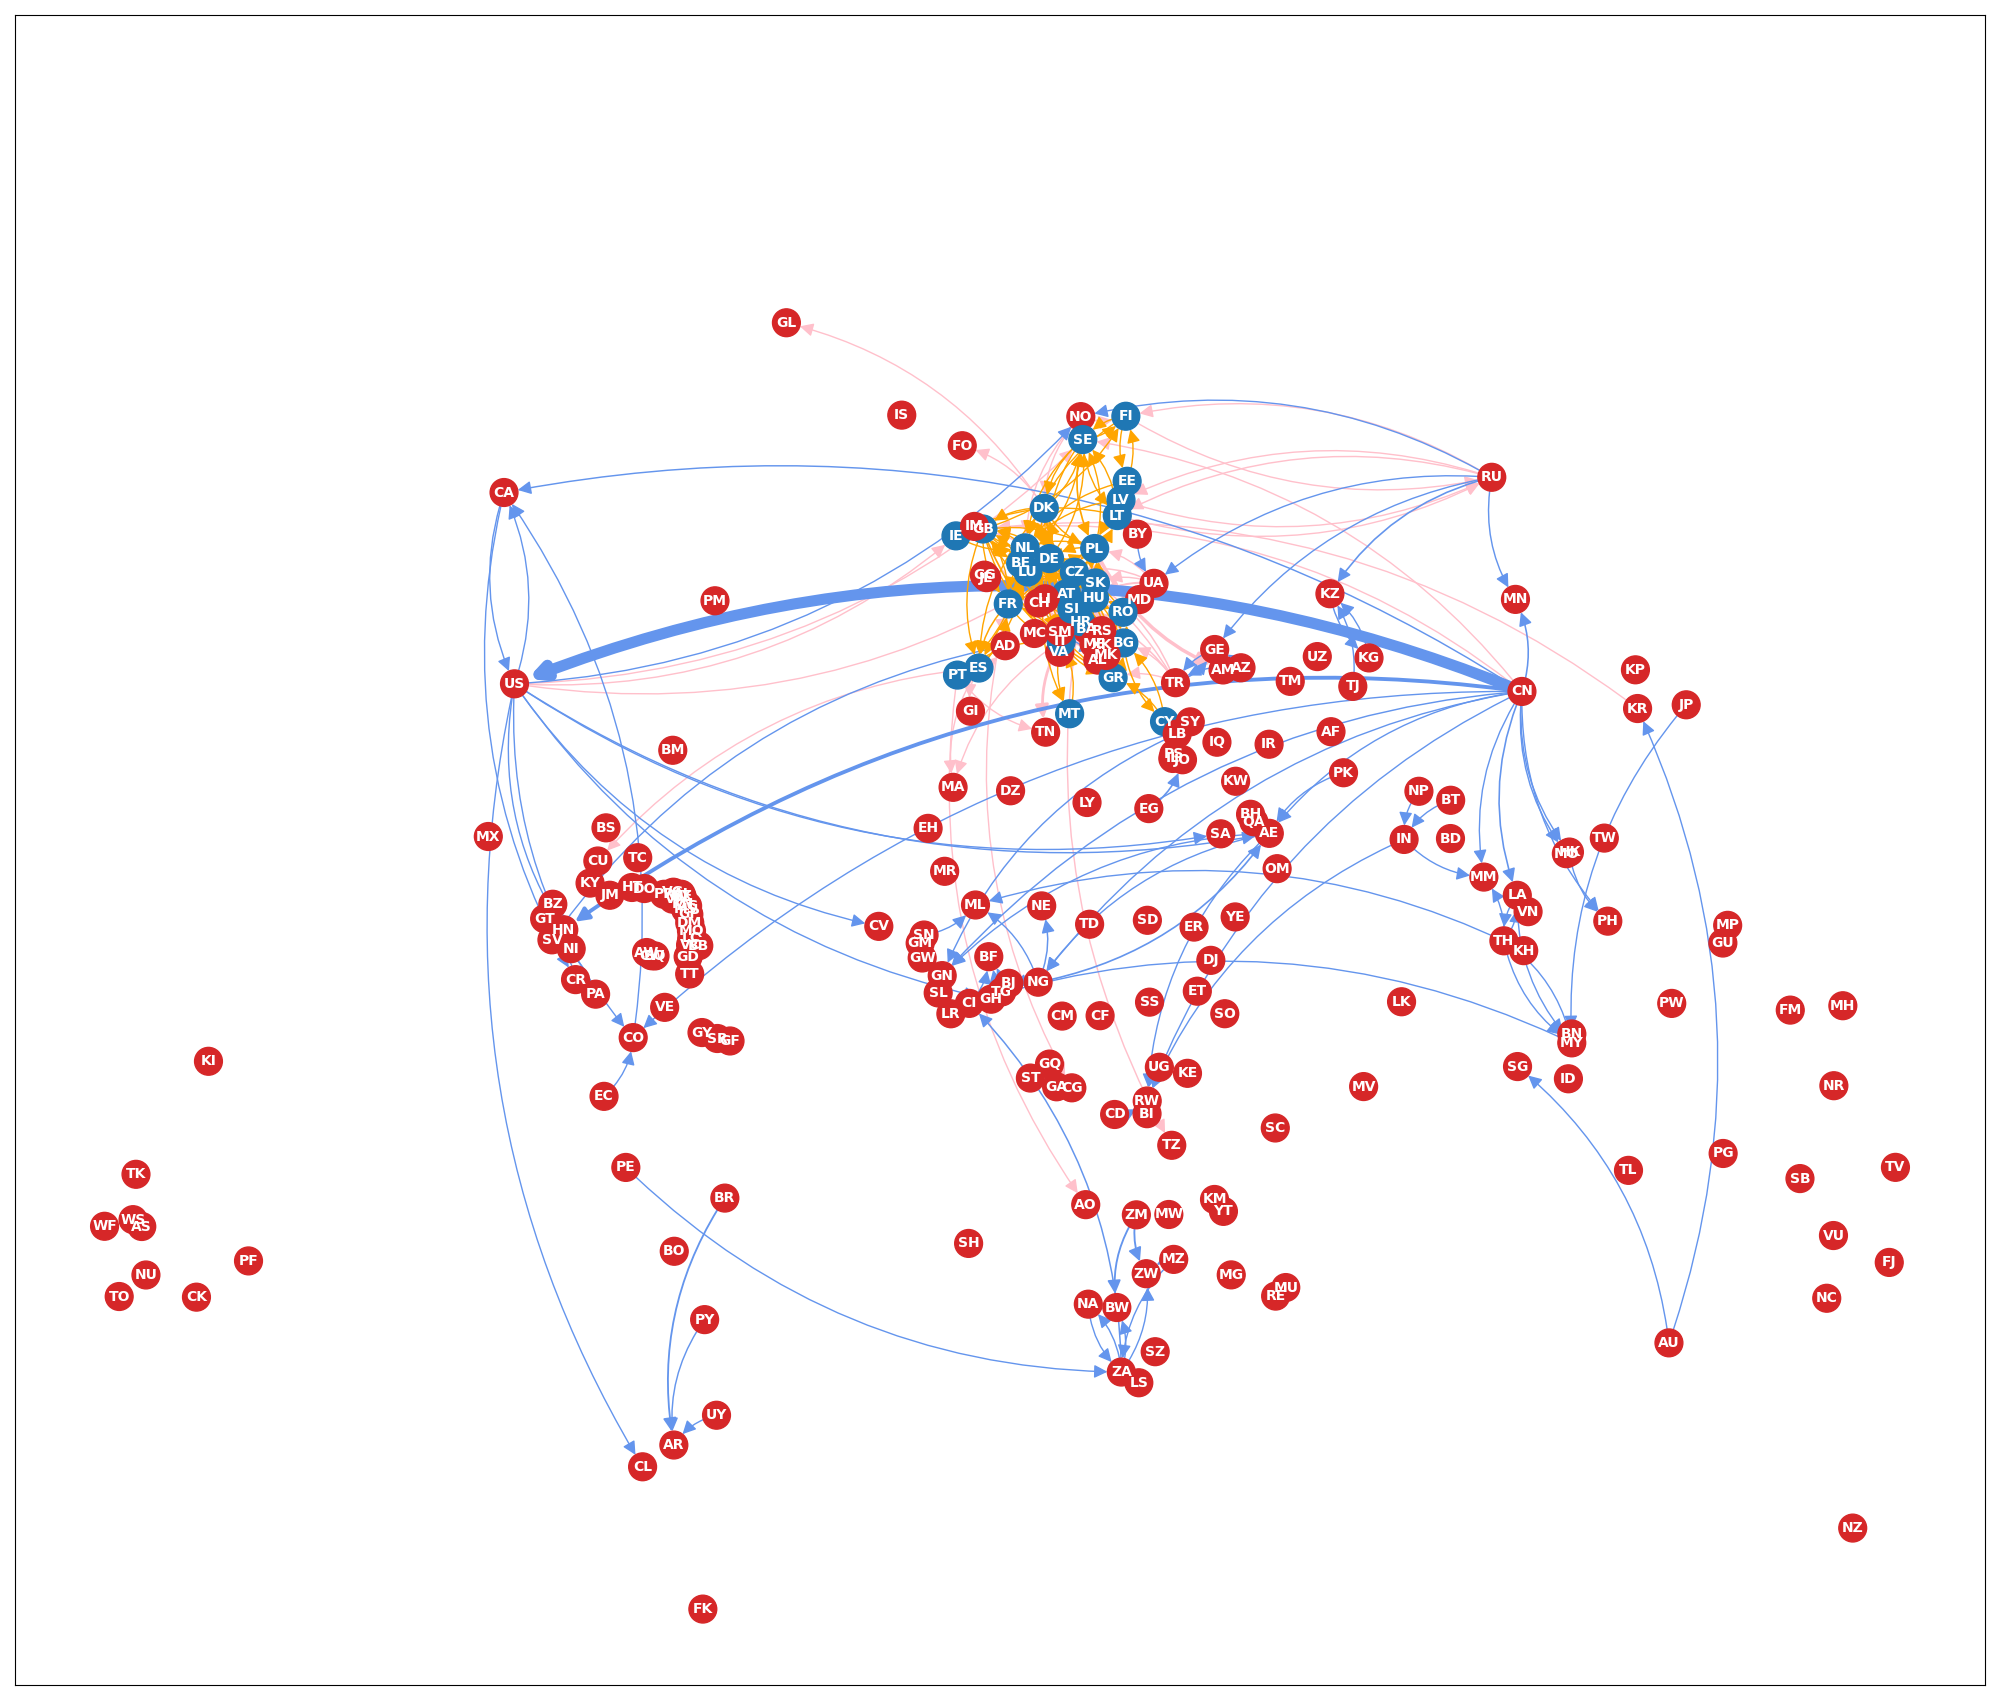
\includegraphics[width=\textwidth]{pics/full_y19_p35_force_79.png}
        \caption[Trade network for \textit{Electricity, gas, steam and air conditioning} in 2019]{Trade network for \textit{Electricity, gas, steam and air conditioning} in 2019, with countries located according to their geographical position.}
        \label{fig:elecgeo}
    \end{subfigure}
    
    \begin{subfigure}{0.5\textheight}
    \centering
        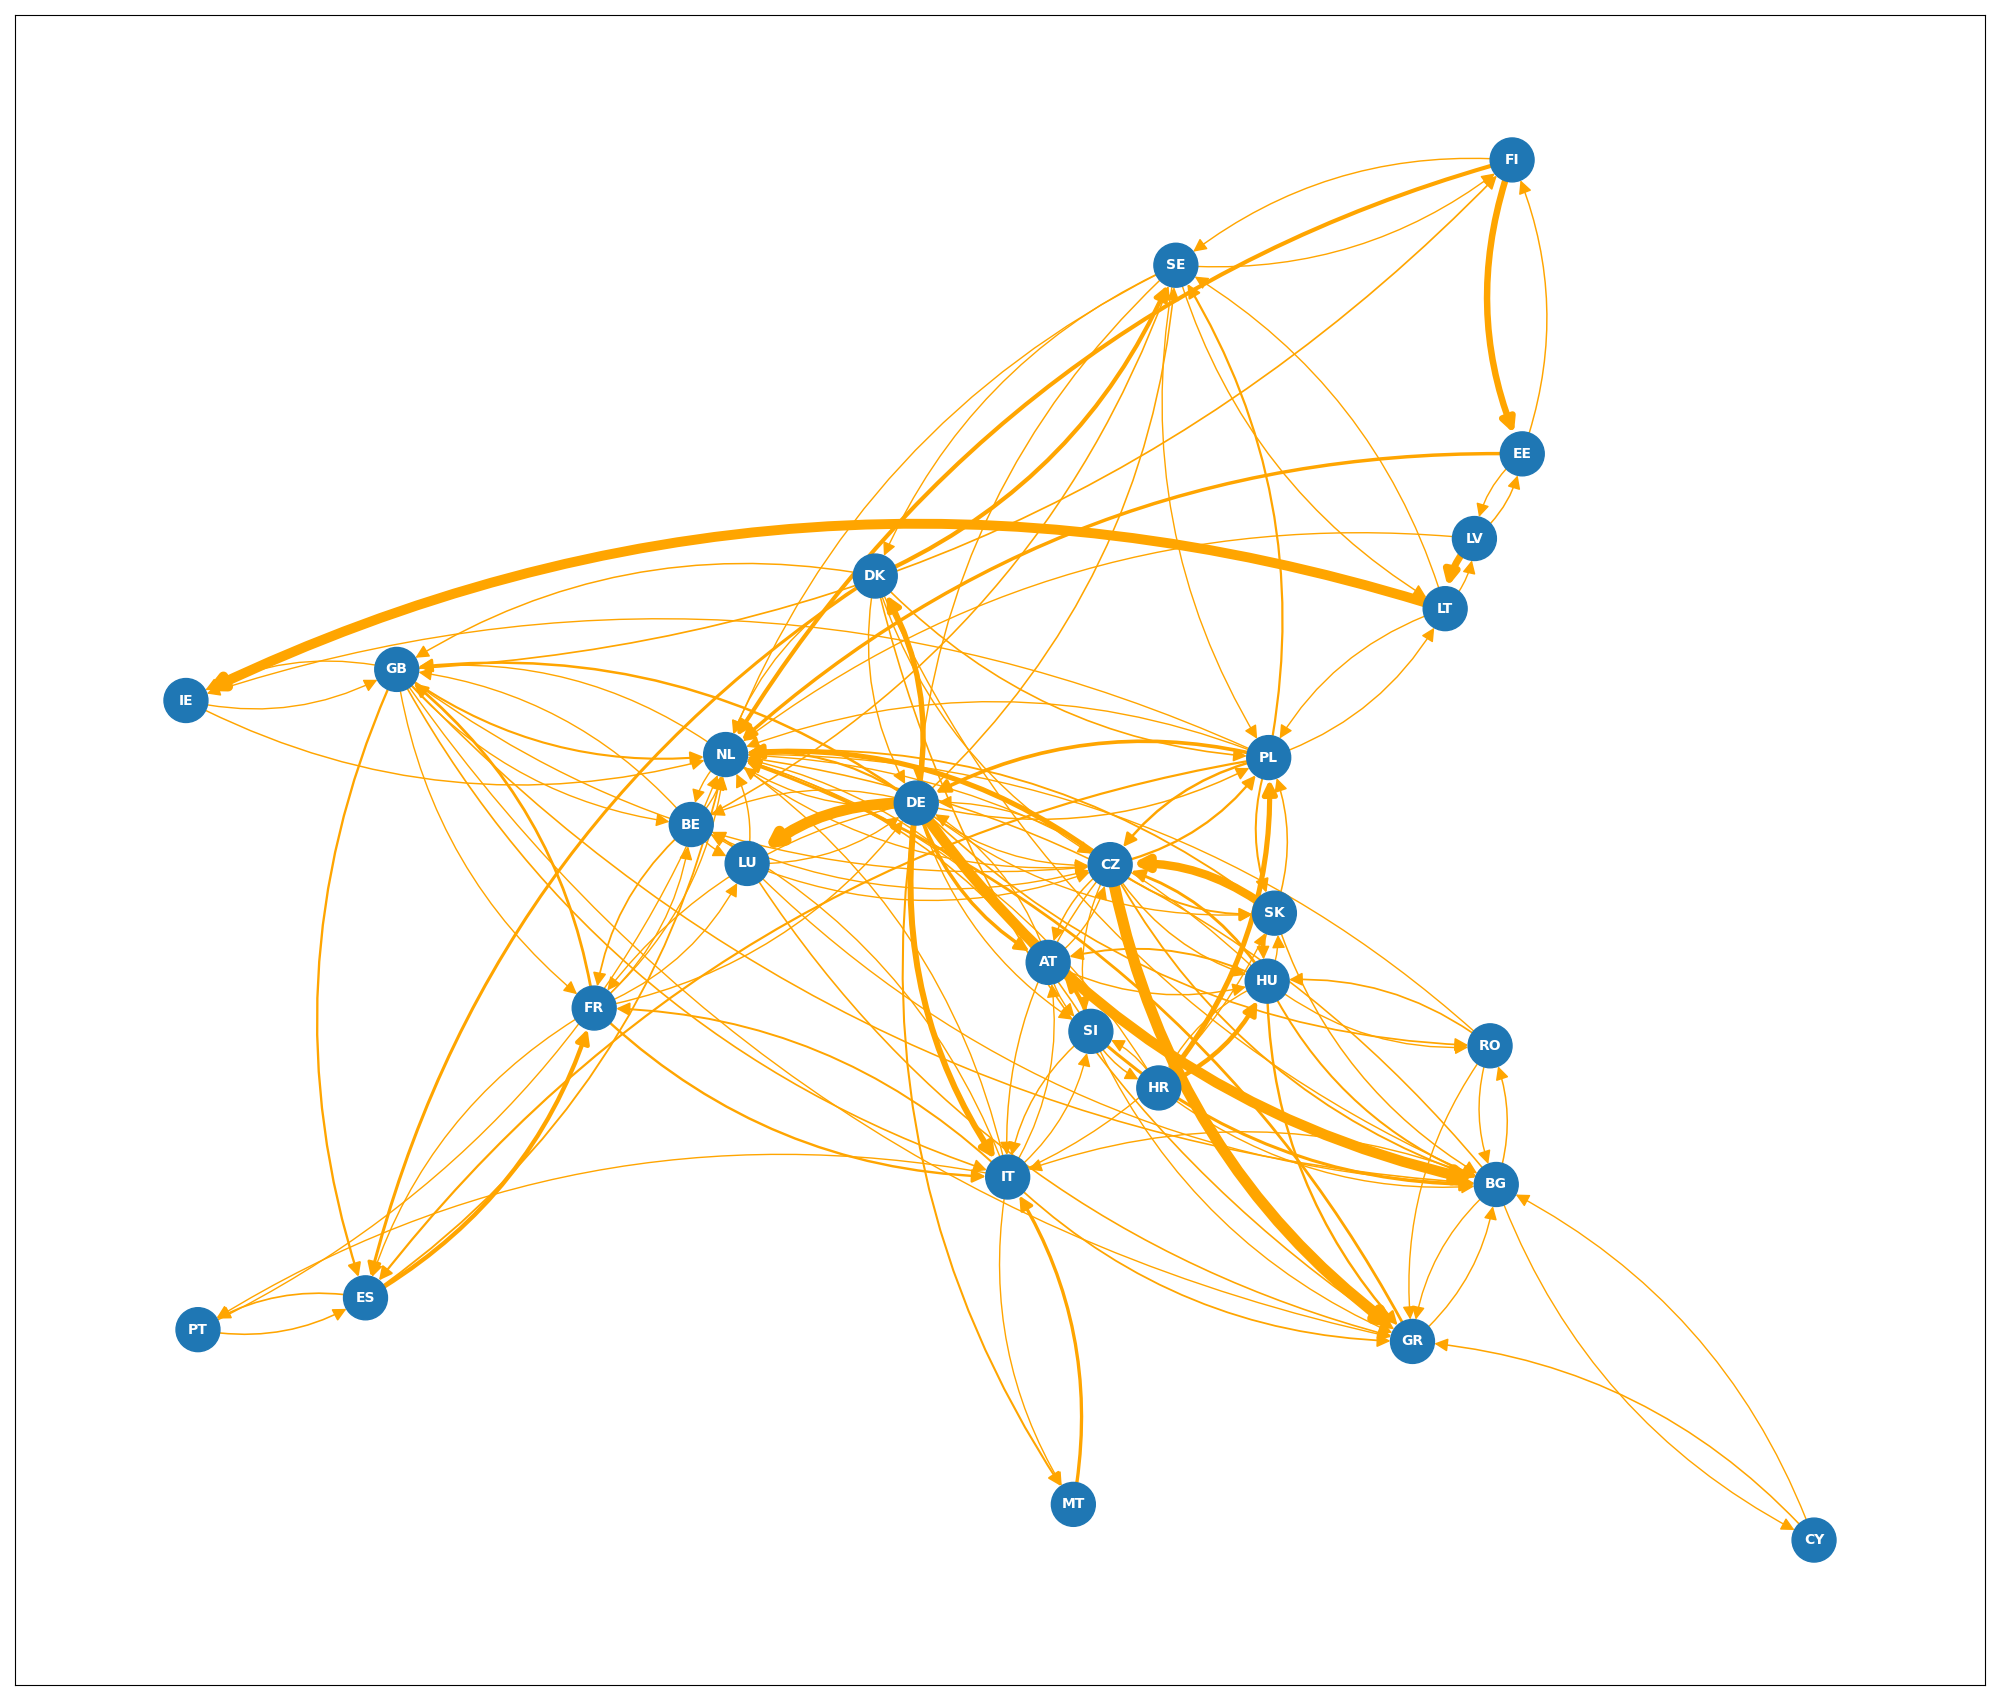
\includegraphics[width=\textwidth]{pics/full_y19_p35_force_82.png}
        \caption[Trade network for \textit{Electricity, gas, steam and air conditioning} in 2019 among European countries only.]{Trade network for \textit{Electricity, gas, steam and air conditioning} in 2019 among European countries only, with countries located according to their geographical position.}
        \label{fig:elecgeoeur}
    \end{subfigure}
    \caption{Caption}
    \label{fig:elecnetwork}
\end{figure}

% FOOD PRODUCTS
\section{The \textit{Food Products} Trade Network}

% - Food network abbastanza interessante perchè aveva size grossa, facilmente interpretabile
The market of \textit{Food Products}\footnote{
    From the EU Economic Activity Classification:
    "This division includes: a variety of products that are the effect of farming, forestry, hunting and fishing, such as meat, fish, fruits and vegetables, fats and oils, dairy products, grain mill products, animal feeds, and other food products intended for humans or animals; semifinished products that are not directly food products; by-products of different value in use (e.g. the hides, oil-cake from the production of vegetable oils); treatment of slaughterhouse waste/waste seized at slaughterhouses/for the production of animal feed."\cite{eurostat2022website}
} is particularly interesting since it is one of the biggest in terms of amount of money exchanged. Moreover, its relationships may be easier to interpret, as they are strongly dictated by the geographical position, soil and climate conditions of countries, that are the main reason why some territories need to import many goods if they want to guarantee diversification in nutrition. Global food trade is of crucial importance for countries since it guarantees food security and availability. Studying the structure of this network allows understanding its vulnerability in terms of food security. Indeed, the interdependencies in food supply, which one can study analytically from trade data, can expose countries to supply risks, especially in periods of global stress, political instability or natural disasters \cite{wang2021evolution}. I will show how, using the method described in previous chapters, one is able to get an understanding of the dynamics of this network. With the data at the hand, the first thing one can do is to look at the graph metrics for this category and how they evolved over time, which provides a first impression of the evolution of the market. Figure \ref{fig:foodmetrics} shows four metrics as time series: size (sum of the weights), average degree, median page rank and average clustering coefficient. We can have a look at the time series to spot trends and variations that can be linked to the latest historical events. Indeed, in the upper left box, we can easily spot the huge drops in the size of the graph that happened during the 2008 financial crisis and the COVID crisis. 
Moreover, regarding 2020, we can see in the two plots on the right the effect of closing the borders to contain the pandemic: the average degree had an important drop since countries truncated or reduced a significant number of exchanges. This is an evidence of the contraction in food trade caused by the sudden outbreak of COVID in 2020, when, for example, some big exporters, suspended or banned grain exports.
At the same time, the steep increase in clustering can be attributed to it being inversely correlated with the average degree: when a node has fewer neighbors the denominator of Equation \ref{eq:clustering} decreases, and so the clustering coefficient goes up, even though the network as a whole may be less connected.
Lastly, in the bottom right plot we see the median page rank among nodes, and we can observe that it used to have a positive trend until 2013, but since then it had started to go down, even more so during COVID. This could be a signal of the market going from a slightly more centralized structure to having more producers and exporters.

\begin{figure}[H]
    \centering
    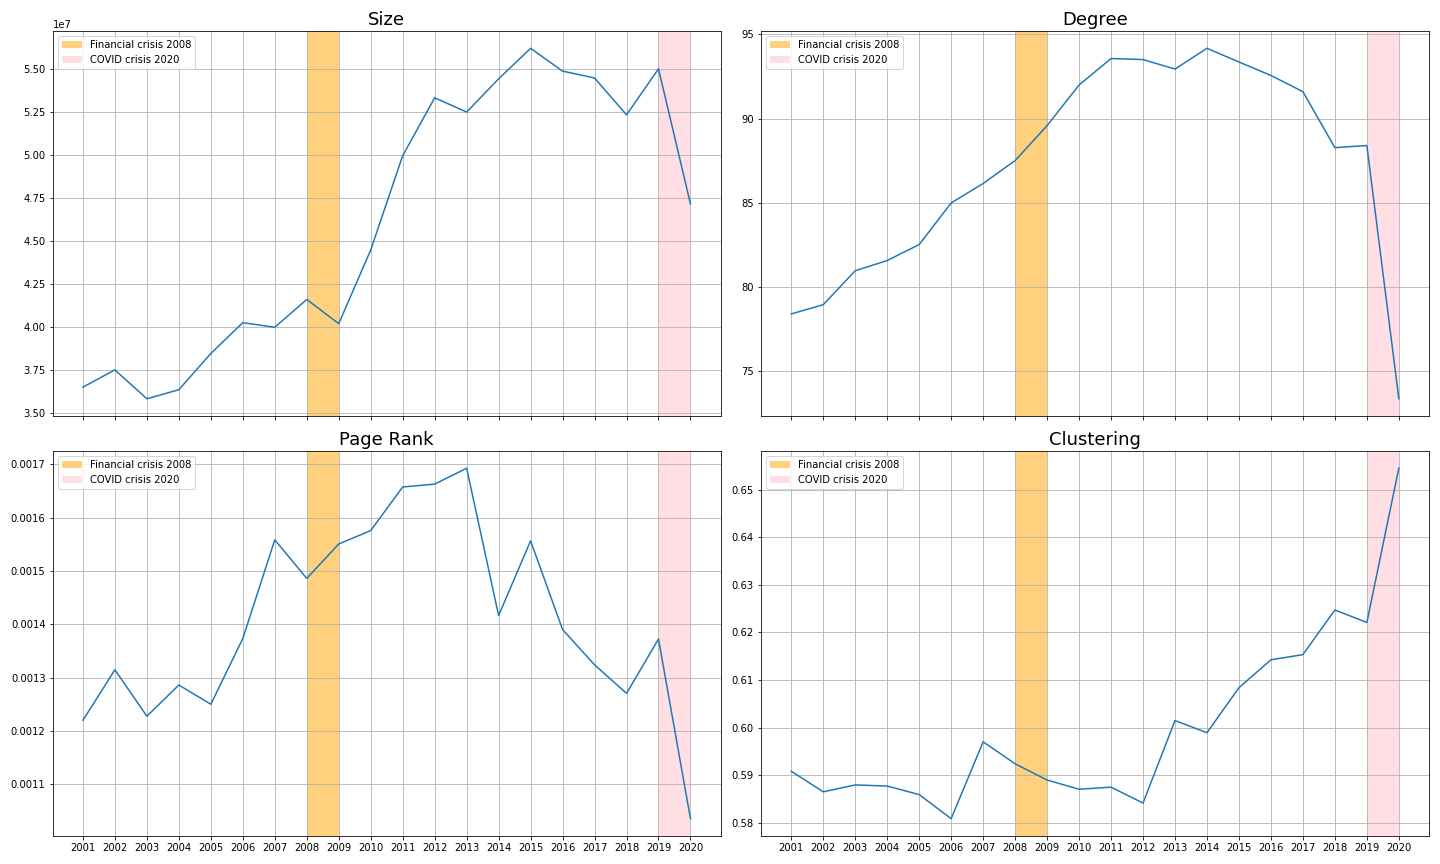
\includegraphics[width=\textwidth]{pics/full_p10_metric_ts.png}
    \caption{Food Metrics TODO}
    \label{fig:foodmetrics}
\end{figure}

\subsubsection*{Degree distribution}

Moving on with the analysis of the trade networks of the Food Products category, one can study the properties of the degree distribution of the graphs over time. As mentioned in Section \ref{sec:4powerlaw}, we can try to verify whether the networks show features of the scale-free property, that is whether there are just a few countries with a high number of trade flows. The procedure to check this is to fit a power law distribution $\alpha k^{-\gamma}$ on the degree distribution (or equivalently fit a simple linear regression on the log-log plot of the distribution) and check how well it fits. I have reported the results in Figure \ref{fig:fooddegree}. The four plots correspond to the four types of degree distribution that I can construct on a directed weighted graph, using in/out, weighted/unweighted degree. In each of these plots, it is reported in blue the power law exponent $\gamma$ for each year in my dataset, and in orange the Mean Absolute Percentage Error\footnote{
    $\text{MAPE}(y, \hat{y}) = \frac{1}{n_{\text{samples}}} \sum_{i=0}^{n_{\text{samples}}-1} \frac{{}\left| y_i - \hat{y}_i \right|}{\max(\epsilon, \left| y_i \right|)}$
} of the linear regression fit on the log-log plot. The MAPE should give us an idea on how well the power law is fit on the distribution: for example, we see that over all the years the fit for the \textit{in weight degree} is better than the one for the \textit{out weight degree}, meaning that there are just a few countries that import high amounts of goods per 1000 inhabitants, while the major exporters are not just a few. Considering instead $\gamma$, we see that the fit on the \textit{in degree} yields a generally lower exponent than the \textit{in weight degree}, meaning that in the former case the hyperbole is less steep than in the latter. 
\begin{figure}
    \centering
    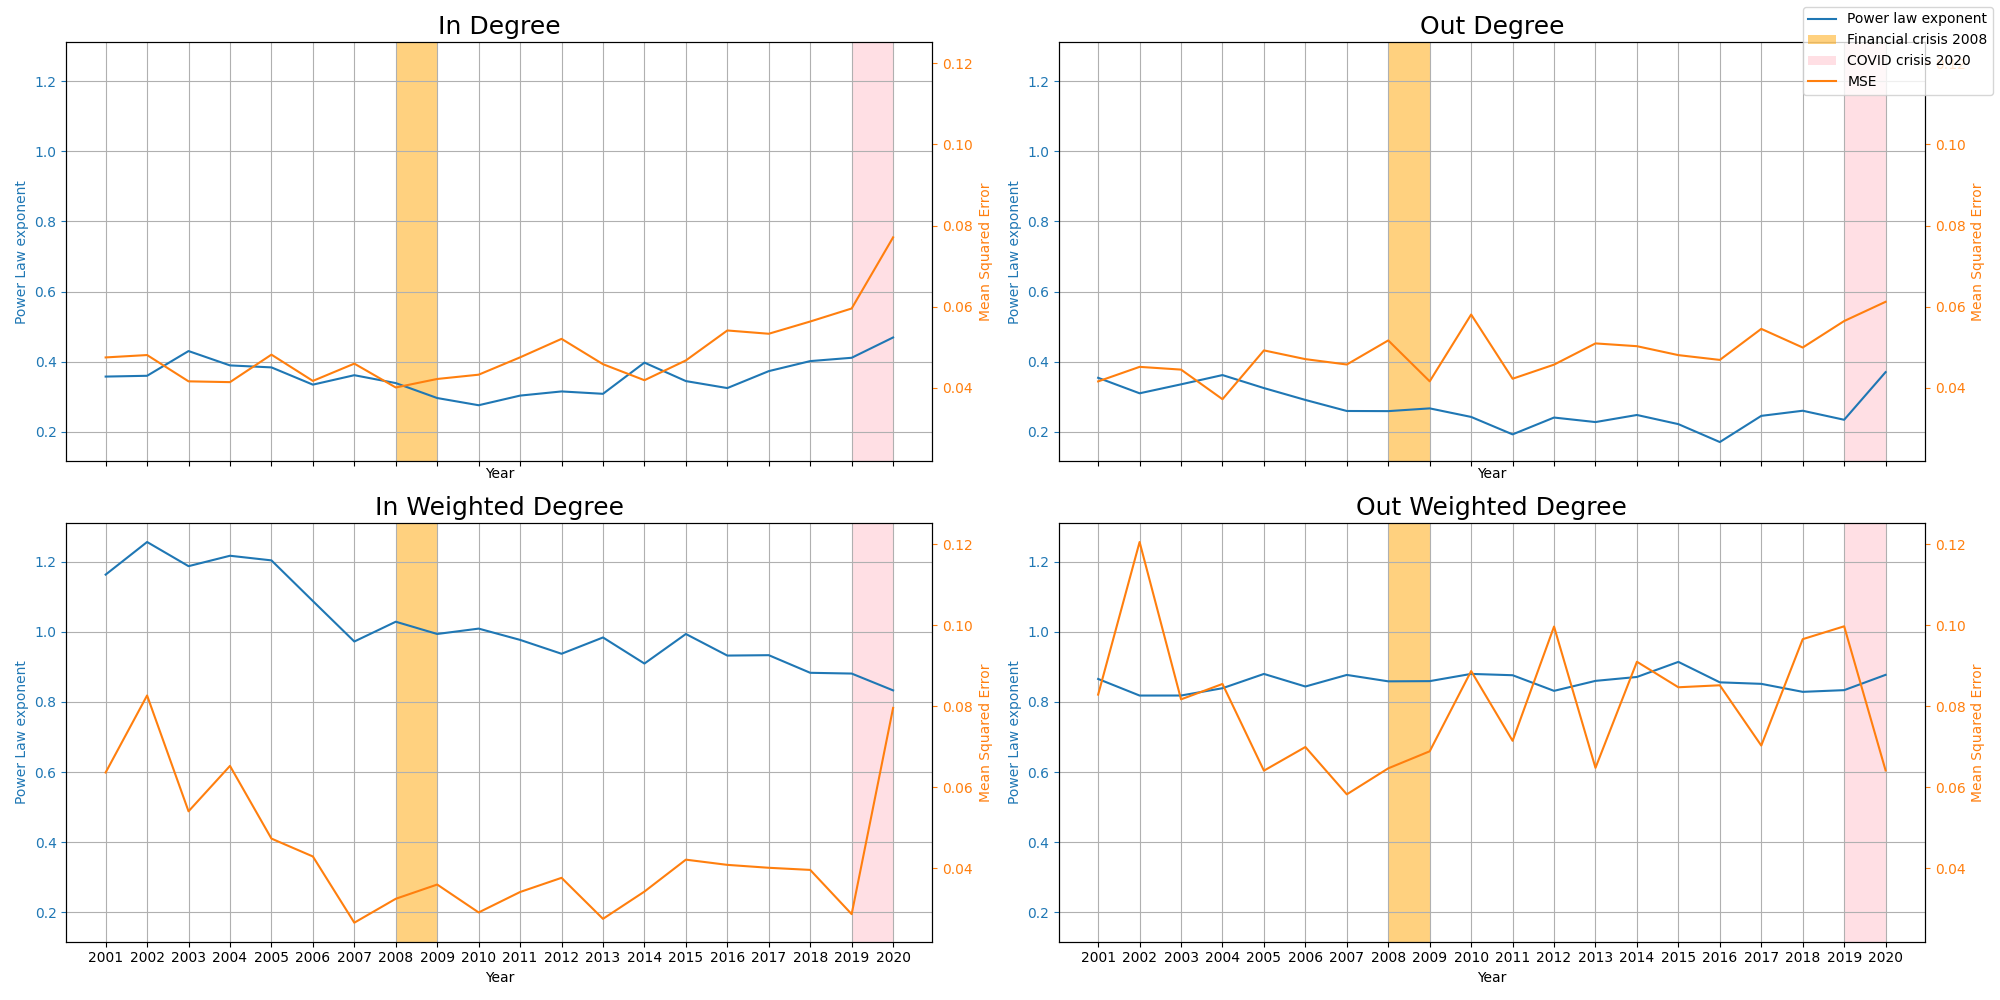
\includegraphics[width=\textwidth]{pics/ts_p10.png}
    \caption{Power law exponents over time of four degree distributions in the Food Products networks.}
    \label{fig:fooddegree}
\end{figure}
To better visualize this, let me choose a suitable year from the time series, for example 2010 which has a lower MSE, and let me plot the degree distribution of that year with its corresponding power law fit. This is shown in Figure \ref{fig:plfood} for the \textit{in degree} and Figure \ref{fig:plfoodw} for the \textit{in weight degree}. In each of these figures we see on the left the degree distribution as the blue dots, while the red curve is the fitted power law; on the right instead we have the same plot but with log-log axis, where the red curve becomes a straight line.
It is quite evident from these pictures that the distribution for the unweighted \textit{in degree} doesn't follow a power law distribution (hence the poor fit) and thus we conclude that this kind of unweighted network is not scale-free. When we look instead at the distribution of the \textit{in-strength}, we observe a better fit: this means that in the trade network for Food Products a high number of countries imports small quantities of goods relatively to their population, while instead a smaller portion of countries are less self-sufficient, and thus they have bigger imports. In short, this is not the case of a few countries occupying a large number of trade flows, but of just a few countries importing a high share of the traded goods.

\begin{figure}
    \centering
    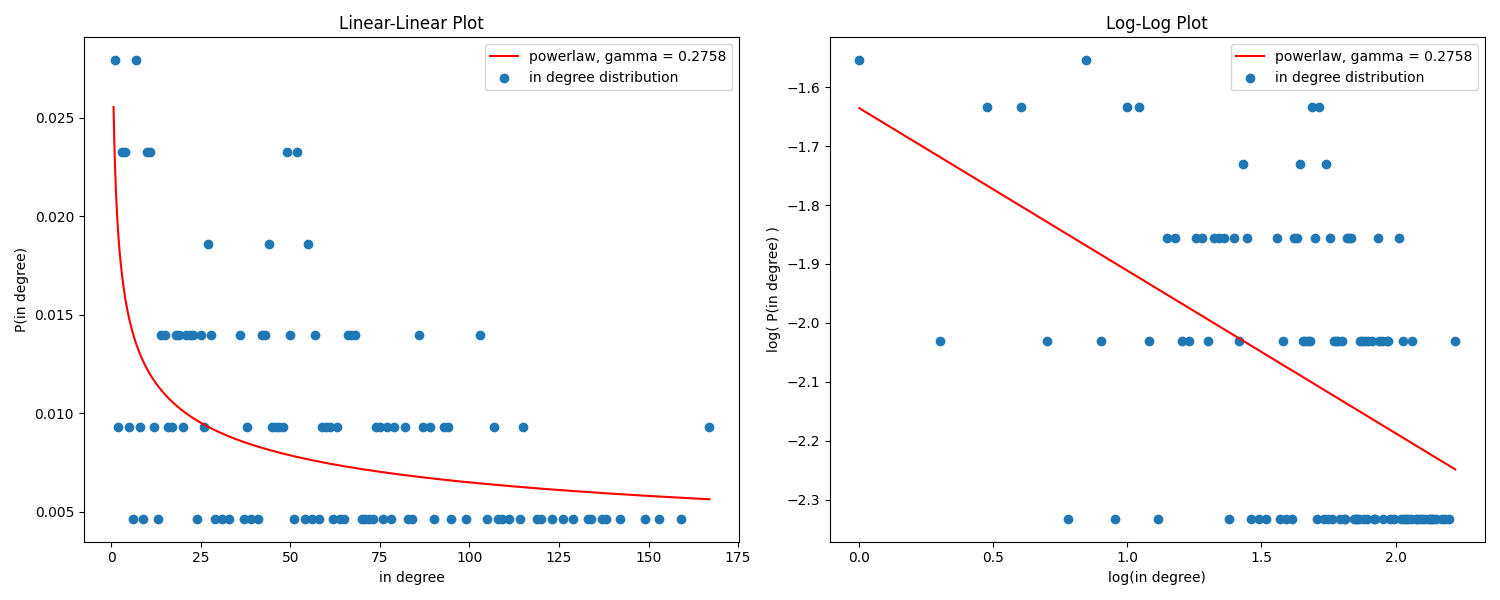
\includegraphics[width=\textwidth]{pics/powerlaw_in_degree_p10_y2010.png}
    \caption{Food Products trade network's degree distribution of the \textit{in degree} in 2010, with power law fit.}
    \label{fig:plfood}
\end{figure}

\begin{figure}
    \centering
    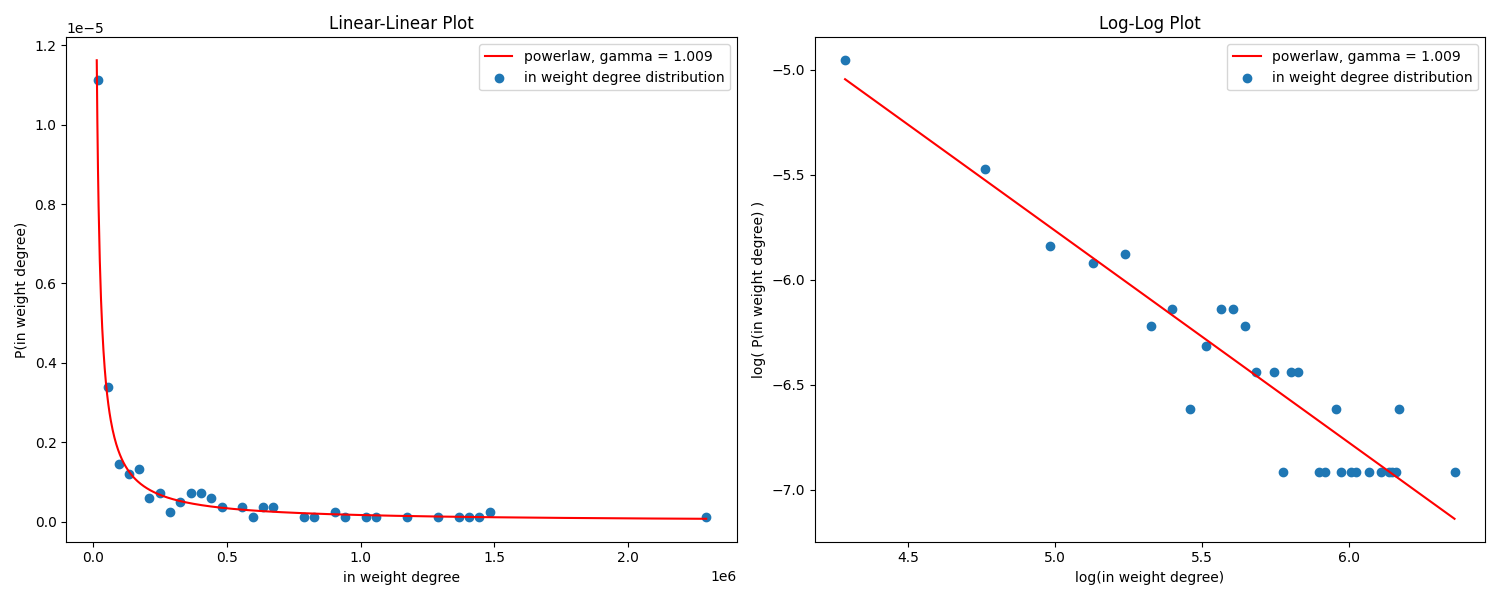
\includegraphics[width=\textwidth]{pics/powerlaw_in_weight_degree_p10_y2010.png}
    \caption{Food Products trade network's degree distribution of the \textit{in weighted degree} in 2010, with power law fit.}
    \label{fig:plfoodw}
\end{figure}

\subsubsection*{Network plot and node properties}

Let us also show the actual network in 2010 with nodes and edges, using the force-directed algorithm. The plot is shown in Figure \ref{fig:foodnetwork}. The first thing we notice here, thanks to the spring layout, is that the graph has a core-periphery structure. Most of the major economies are at the center of the graph, that is to say, they are the countries which are the top exporters of \textit{Food Products} to other nodes. We can identify them by considering the node size in the picture, which is proportional to the out weighted degree: a node is bigger if the corresponding country exports many goods of this category. At the center we find for example the European countries, which have a dense web of imports (the \textit{orange} exchanges) among themselves, and also a considerable number of exports to the peripheral countries (the \textit{pink} edges). Hence, the layout helps us identify which are the most central countries before looking at metrics: in the \textit{core} of the network we see nodes such as the Netherlands (NL), the United States (US), Germany (DE), Brazil (BR), France (FR), which have a high \textit{out degree}, with a high number of connections with peripheral nodes. If instead we were to look from the perspective of importing countries, we could identify which are the links of strongest dependence, intended here as the ones with the highest weight. These are shown in Table \ref{tab:top10foodimp}. In the top half, among the strongest dependencies, we find the exports from Denmark (DK) to Greenland (GL), from the United Kingdom (GB) to Falkland Island (FK) and from Spain (ES) to Andorra (AD). These are just few examples of territories politically linked to the primary country, and thus historically depending on it for the economy. The strongest incoming links for Italy (IT), instead, are reported in the bottom half of the table. We can observe that most of the countries that export the most \textit{Food Products} to IT are EU countries, and also that for this specific category the level of dependence is not as high as that of the ones in the top half of the table.


\begin{figure}
    \centering
    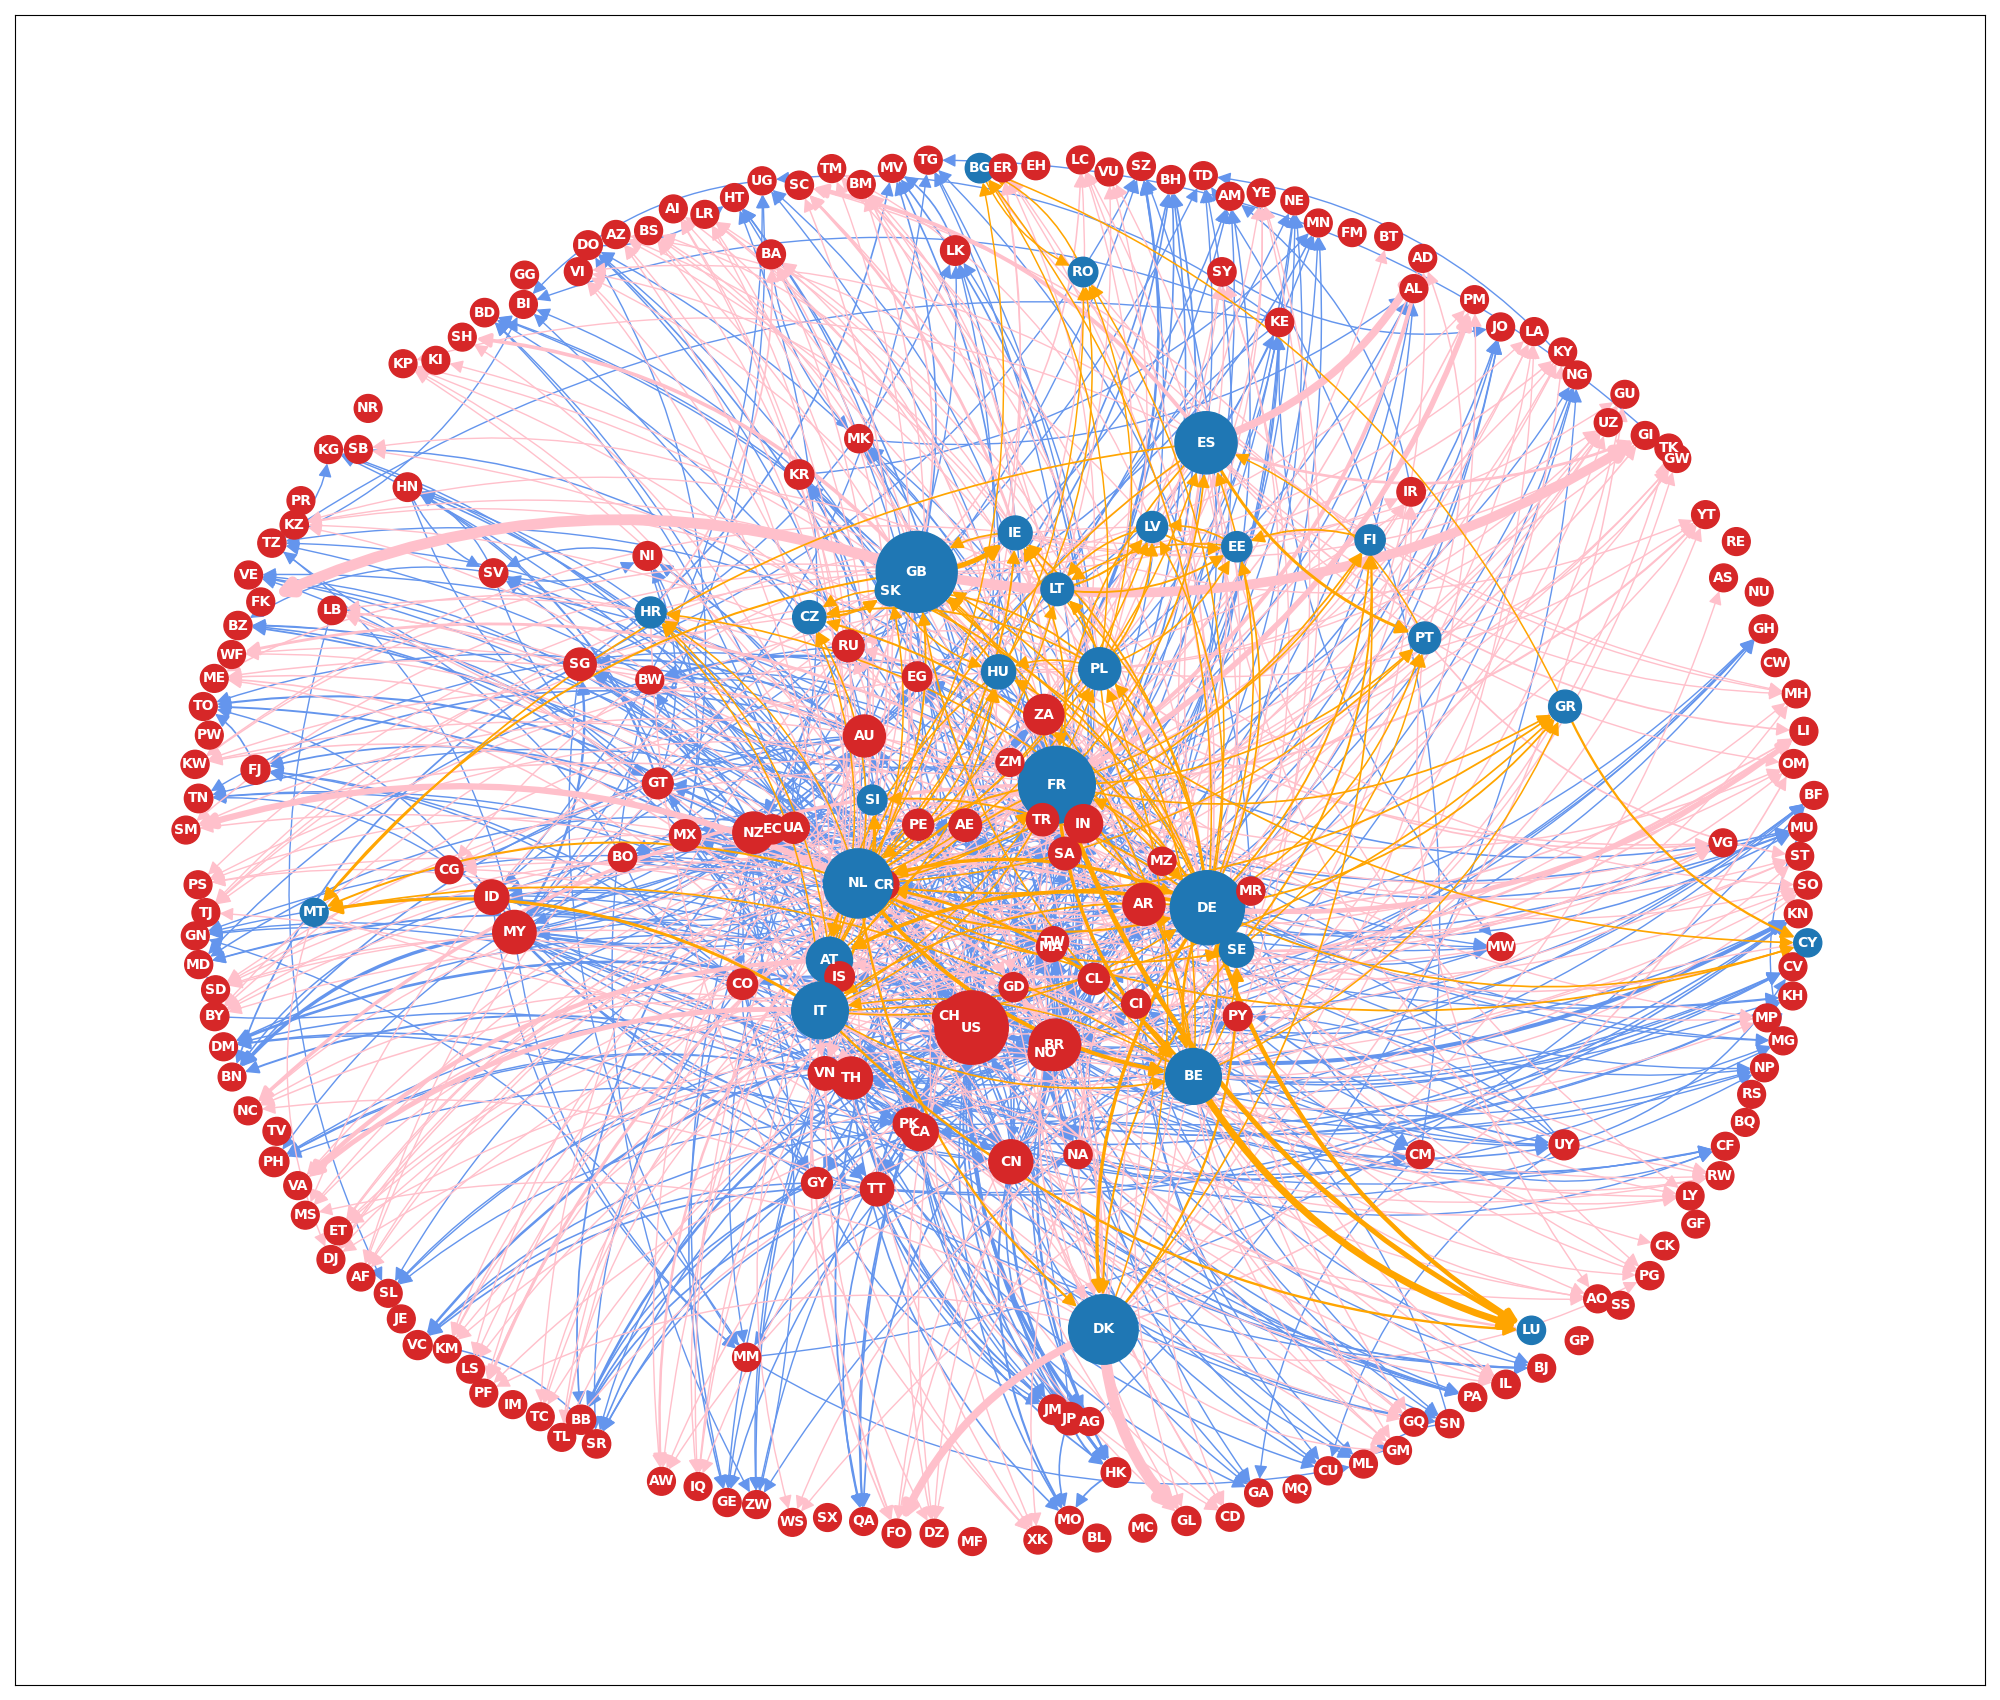
\includegraphics[width=0.8\textwidth]{pics/full_y10_p10_force_116.png}
    \caption[Global trade network of \textit{Food Products} in 2010.]{Global trade network of \textit{Food Products} in 2010. The size of the node represents the \textit{out-strength} of that country. The color of the node indicates EU countries (\textit{blue}) and non-EU (\textit{red}); the color of the edge is \textit{orange} for intra-EU exchanges, \textit{pink} for EU - non-EU exchanges and \textit{azure} for extra-EU exchanges. Only the top 5 import partnership for each country are shown.}
    \label{fig:foodnetwork}
\end{figure}

\begin{table}
    \centering
    \begin{tabular}{llr}
\toprule
Country From & Country To & Value €/1000 p. \\
\midrule
          DK &         GL &      1463214.81 \\
          GB &         FK &      1426621.59 \\
          GB &         GI &      1235017.11 \\
          ES &         AD &       953921.43 \\
          DK &         FO &       947595.33 \\
          BE &         LU &       836591.73 \\
          NL &         SM &       735949.98 \\
          FR &         PM &       623087.90 \\
          FR &         LU &       542263.65 \\
          GB &         IE &       536479.49 \\
\midrule
          DE &         IT &        69071.78 \\
          FR &         IT &        52386.18 \\
          ES &         IT &        43262.14 \\
          NL &         IT &        30148.72 \\
          BE &         IT &        14596.66 \\
          AR &         IT &        13405.36 \\
          AT &         IT &        12854.69 \\
          DK &         IT &        10292.91 \\
          PL &         IT &         8509.97 \\
          GB &         IT &         8066.08 \\
\bottomrule
\end{tabular}
    \caption{Top 10 edges by weight in the \textit{Food products} market and top 10 incoming edges for Italy (IT) by weight, in 2010.}
    \label{tab:top10foodimp}
\end{table}

Let's consider now a specific country and have a look in detail at its position in the network and over time. In Figure \ref{fig:nedmetrics}, I considered the Netherlands (NL) and showed the main node properties. What is surprising to see is that although NL was one of the main exporters of \textit{Food Products} in 2010, we learn from this plot that since then both its \textit{out degree} and \textit{out strength} have been going up even more, meaning that the country has intensified its exportation output [CITARE GOVERNO NL]. The high value of out degree is consistent with the low values of Page Rank and authority values: given how these metrics are defined, it was to be expected, since NL has a lot of out going edges. Furthermore, a consideration can be made about the values of Hub, Out Degree and Clustering Coefficient. Although NL had higher values of Hub in the early years, after 2007 it has remained stable at low levels. This seems in contradiction with the increase in out degree, since one would expect a node with many connections to be a hub. However, this phenomenon can be explained by the simultaneous decrease in clustering coefficient: in fact, if the acquired out going connections of NL are all pointing towards peripheral countries, which have no connections among them since they don't act as exporters, and also they have low authority value since they don't buy goods from many other hub countries, then the hub value of NL itself is justified to stay stable at low values.

\begin{figure}
    \centering
    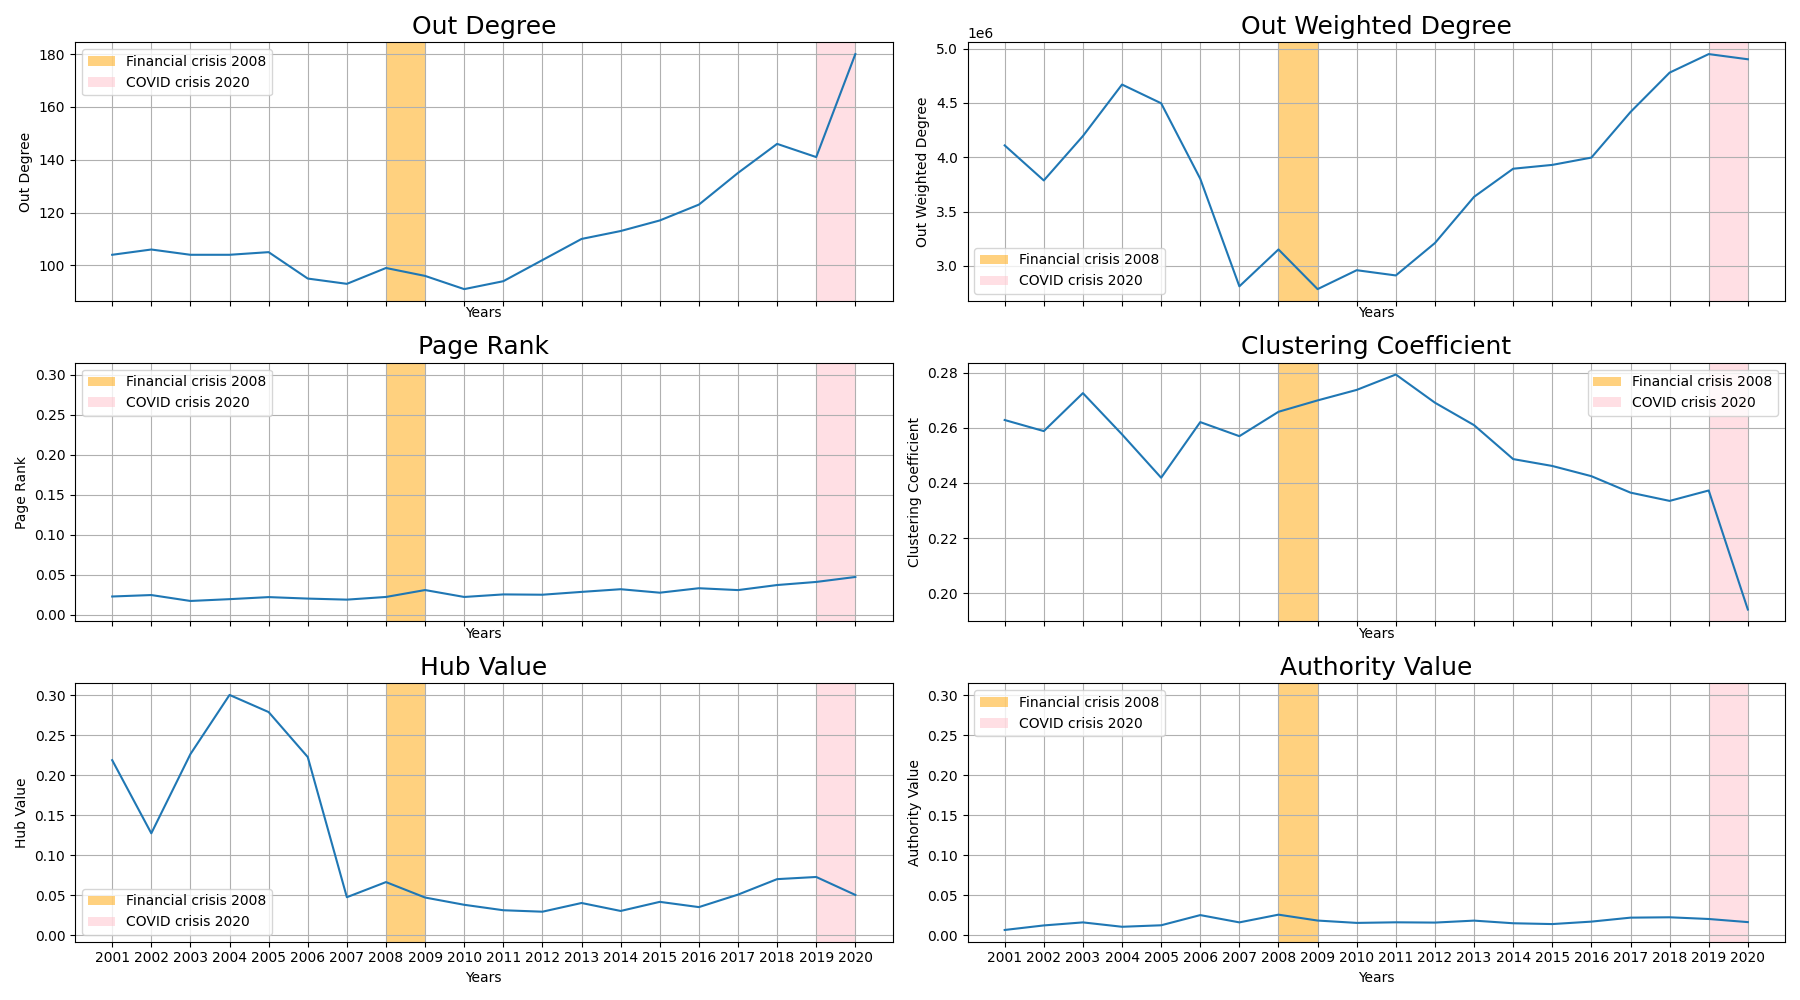
\includegraphics[width=\textwidth]{pics/NL_p10_metric_ts.png}
    \caption{Network metrics for the Netherlands (NL) of the trade market of \textit{Food Products} over the years.}
    \label{fig:nedmetrics}
\end{figure}

% \pagebreak
\subsubsection*{Community detection}

An alternative approach to study such trade networks is to understand their block structure. In recent years, this has been a hot topic in the research of network theory applied to real-life graphs. It was stated in previous chapters that the majority of these networks appear to have a \textit{core-periphery} structure, without however supporting the claim with any evidence. In this section, I will apply the methods of Degree Corrected Stochastic Block Model and Louvain Algorithm to the trade network of \textit{Food Products}. Analyzing the outputs of such algorithms can help us better understand the relationships among countries in this sector, and also verify whether the obtained clusters of countries support the idea of a core-periphery network. The two methods I used need to be fed slightly different networks: while for Louvain an extension of the modularity metric for weighted connections exists, for SBM and DCSBM I had to use a binary network, and hence I followed the procedure explained in Section \ref{sec:3binarygraphs}. I have run both algorithms on each available year of the \textit{Food Products} trade network, with the following parameter settings:
\begin{itemize}
    \item DCSBM: $alpha = 0.1$, which is the parameter of the Dirichlet distribution over the vector of probabilities of memberships;
    \item Louvain Method: $resolution = 0.5$, which is the $\gamma$ parameter in the modularity formula (Equation \ref{eq:3deltamod}).
\end{itemize}
Let us start to look at the results from Figure \ref{fig:dcfood}: we have represented here a \textit{parallel categories} plot, in which numbers represent the communities found by the DCSBM algorithm, and the colors refer to the memberships of 2019. We can observe here that the method has identified 9 blocks in 2019, some of which like 1, 2 and 7 are also quite numerous. The peculiarity of this plot is that it allows us to see where the nodes in each community come from, and if they often changed membership through the years. In particular, while clusters like 1 and 7 have been almost always consistent, we deduce that community 2 is the result of an aggregation of countries that used to belong to many other different communities in past years, and that only from 2017 on they started to get together in a single group. It is worth noting that none of these are formal communities, meaning that the model is agnostic of any trade agreements among groups of countries, as for example the European Union. The algorithm takes only into account all the links of nodes with each other, and tries to identify patterns of countries behaving in the same way or having tight relationships.
Aside from DCSBM algorithm, we can also run the Louvain Method on the graphs, which, contrary to SBM, is a technique created primarily for community detection. In this case, the results are shown in Figure \ref{fig:loufood}. The first thing that we notice here is that the number of communities identified is lower, just three in 2019. The reason for this has to be found in the completely different functioning of the two methods: in fact, while DCSBM searches for nodes with stochastic equivalence, and this may lead to an output with more blocks, Louvain optimizes the modularity metric, which favors bigger blocks given the resolution parameter of $0.5$. Next, we also observe that only the green community (2) has quite preserved itself through the years, while the members of the purple (1) and yellow (3) ones come from different older clusters which have been dismembered.


\begin{figure}
    \centering
    \begin{subfigure}{\textwidth}
        \centering
        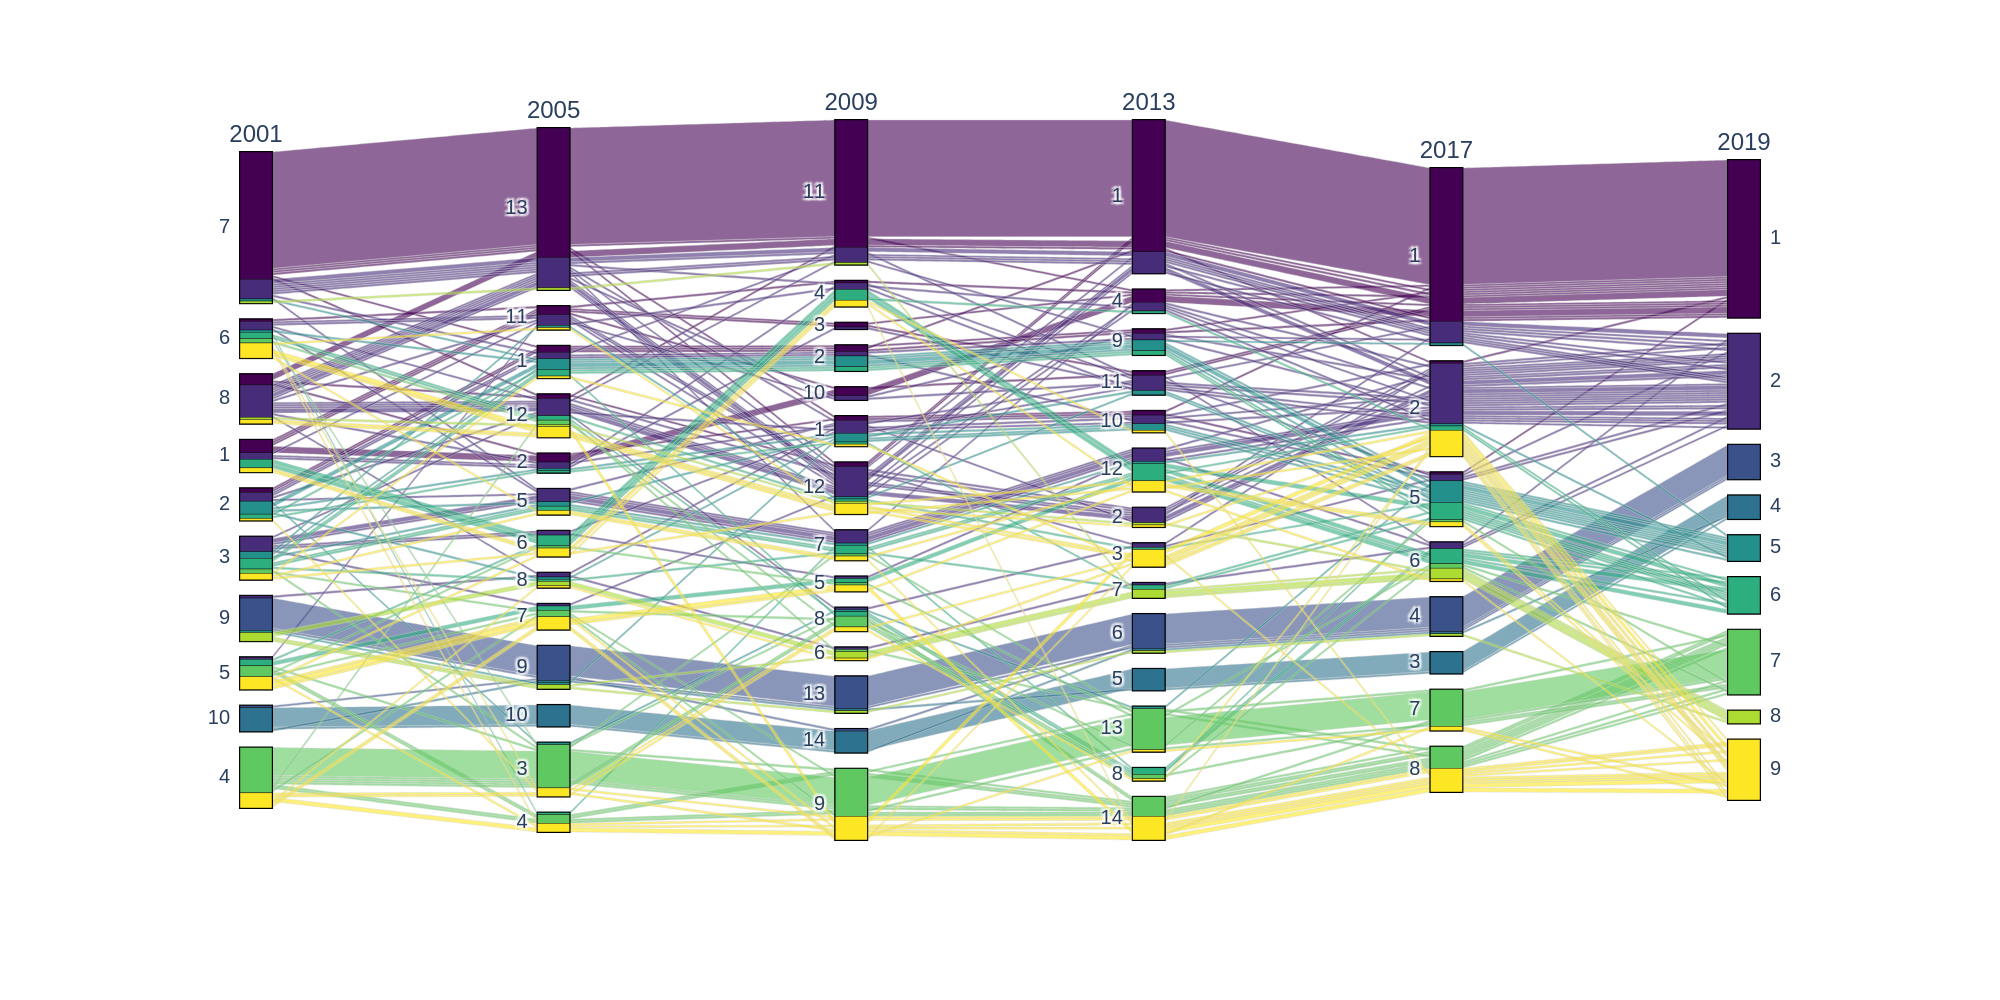
\includegraphics[width=\textwidth]{pics/dc_p10.png}
        \caption[Evolution over time of the communities of the \textit{Food Products} trade network, computed using the Degree Corrected SBM.]{Evolution over time of the communities of the \textit{Food Products} trade network, computed using the Degree Corrected SBM. Communities are shown every 4 years, plus 2019. The colors refer to the memberships in 2019.}
        \label{fig:dcfood}
    \end{subfigure}

    \begin{subfigure}{\textwidth}
        \centering
        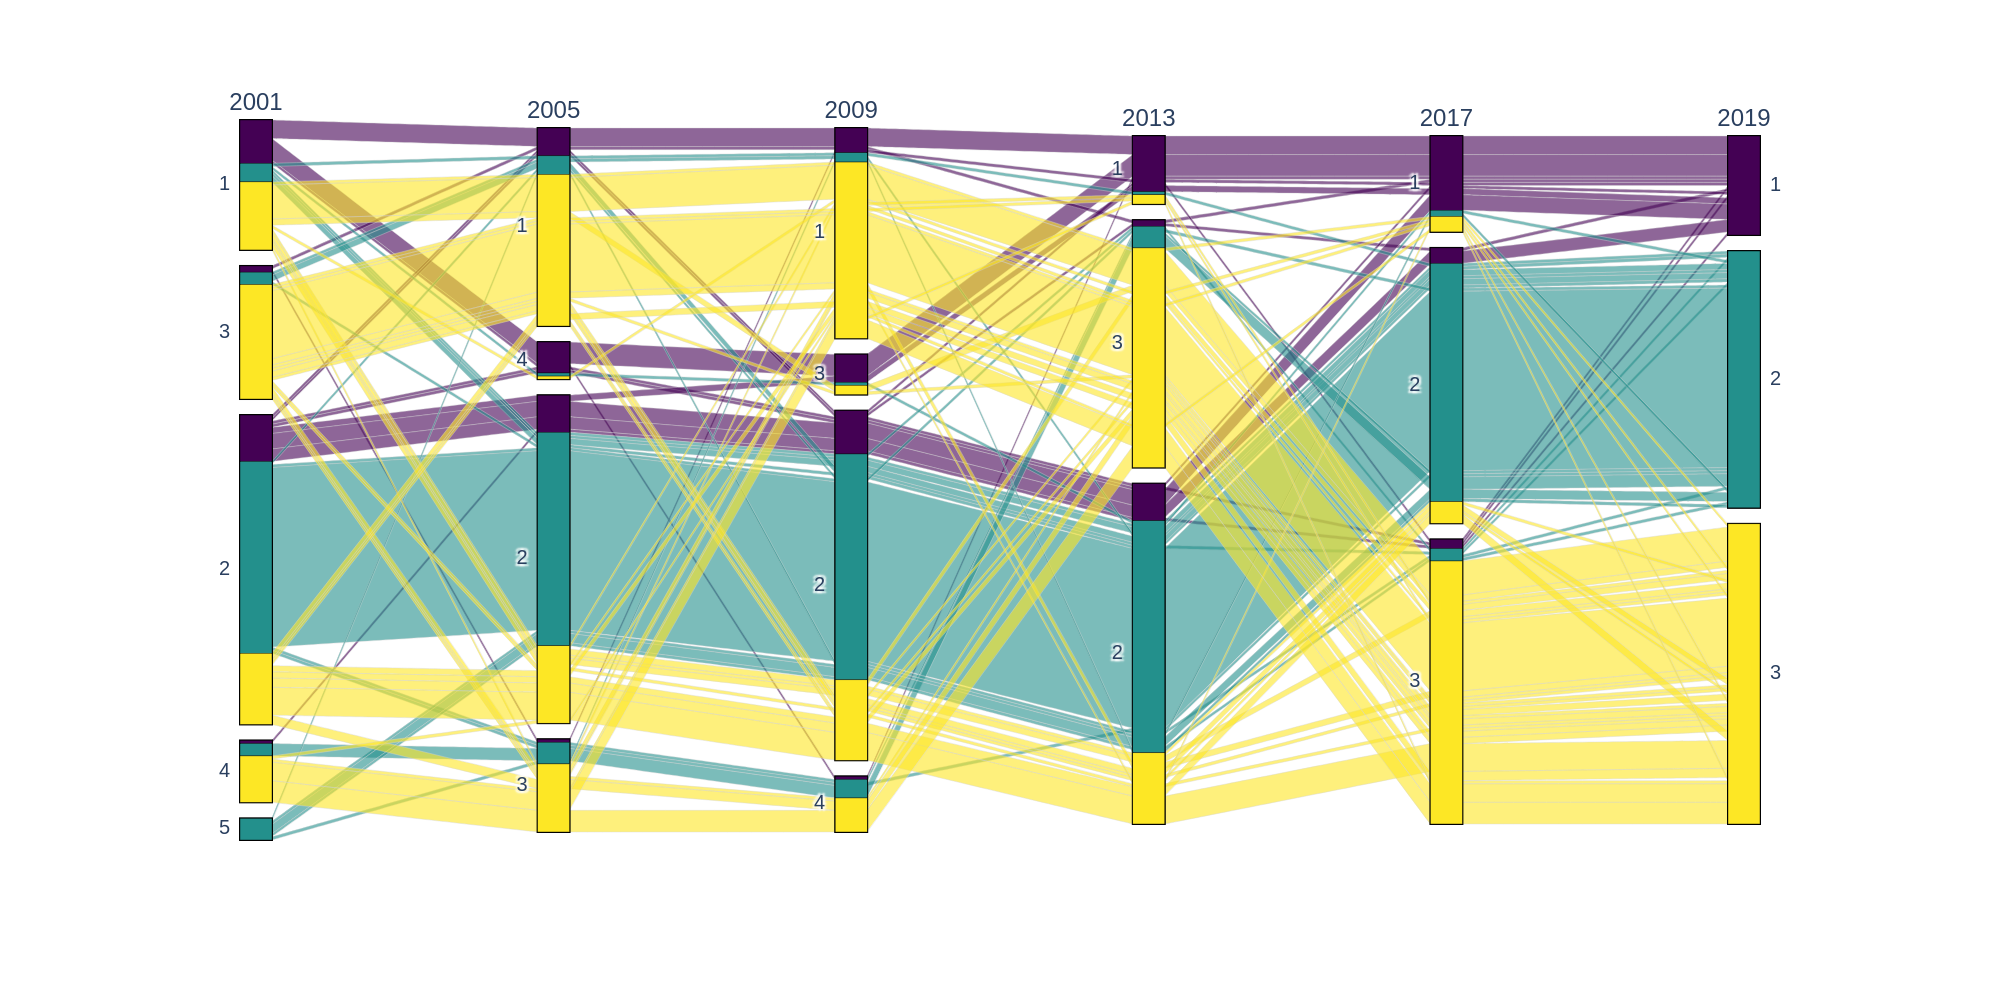
\includegraphics[width=\textwidth]{pics/lou_p10.png}
        \caption[Evolution over time of the communities of the \textit{Food Products} trade network, computed using the Louvain Method.]{Evolution over time of the communities of the \textit{Food Products} trade network, computed using the Louvain Method. Communities are shown every 4 years, plus 2019. The colors refer to the memberships in 2019.}
        \label{fig:loufood}
    \end{subfigure}
\end{figure}

The type of plots like in Figures \ref{fig:dcfood} and \ref{fig:loufood} are only useful to see the evolution of communities in time, and how they formed, but they don't provide us any insight into how these are actually structured. To visualize this, I have taken the membership output in 2019 of both DCSBM and Louvain, and plotted the same network twice, with the communities coded in the colors of the nodes. They are shown in Figure \ref{fig:foodnetworkdc} and \ref{fig:foodnetworklou}, respectively. Considering the first plot, we can say that the result of DCSBM has successfully identified a \textit{core-periphery} structure (the number corresponds to the clusters of Figure \ref{fig:dcfood}): in the middle, we find the blue (3), purple (2) and green (6) communities, which as their position in the spring layout suggests, as well as the size of their nodes, are the major exporters in these sectoral trade network. Moreover, an additional insight can be gained by this community result: if we look carefully at the nodes belonging to the blue (3) and purple (2) blocks, we can see that they are almost all countries of the EU. Their division also, is not without sense: in fact, the former community includes countries such as NL, FR, DE which are big world (and thus EU) exporters, while the latter includes those countries which still trade considerably with the EU and are members, but they don't export as much. The green community (6) of countries instead, could be defined as composed of mainly non-EU countries (like US, TH, NZ) but which are still relevant in the export market for \textit{Food Products}. A similar reasoning can be done for the plot below, where the communities of the Louvain method are displayed, but with a fundamental difference. While in DCSBM peripheral countries are more likely to belong to a community of their own, in Louvain they belong to the same community of the core countries with which they trade the most. In fact, we could say that light green countries (3) exchange highly with EU countries, while the dark green (2) ones trade mostly with non-EU countries. Furthermore, it can be noticed that both DCSBM and Louvain have captured the same community structure as to what it concerns the core exporting countries.

\begin{figure}[H]
    \centering
    \begin{subfigure}{0.8\textwidth}
        \centering
        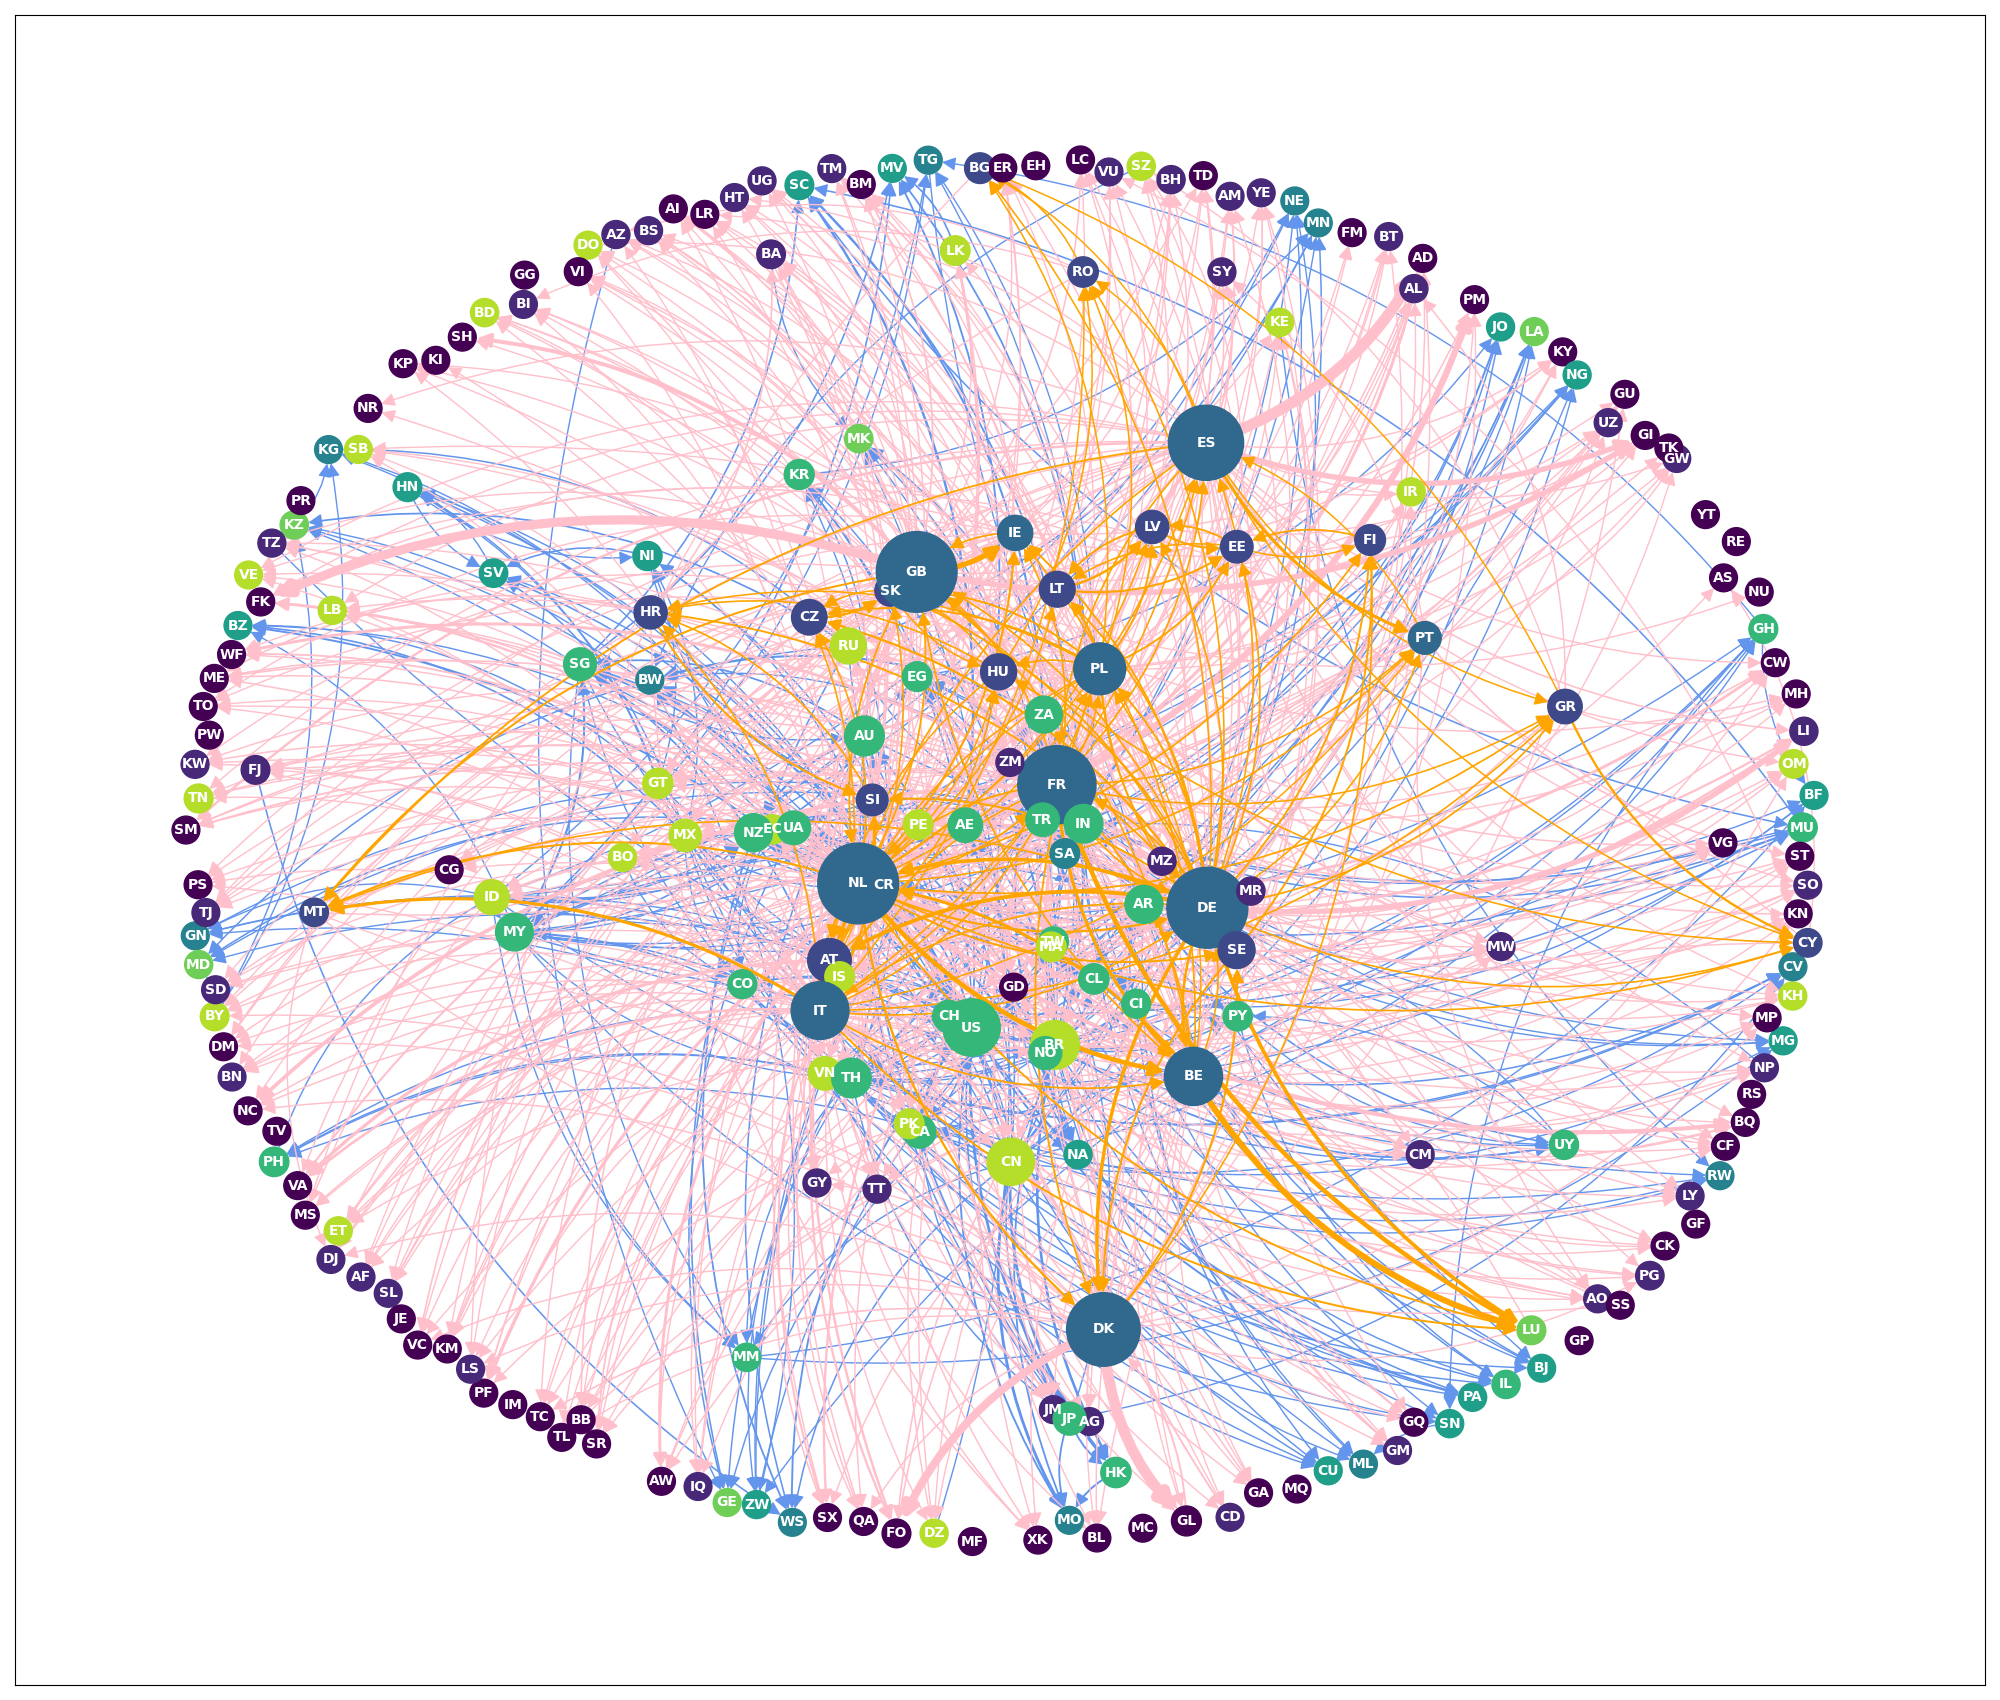
\includegraphics[width=\textwidth]{pics/full_y19_p10_force_143_dc.png}
        \caption{Degree Corrected SBM}
        \label{fig:foodnetworkdc}
    \end{subfigure}

    \begin{subfigure}{0.8\textwidth}
        \centering
        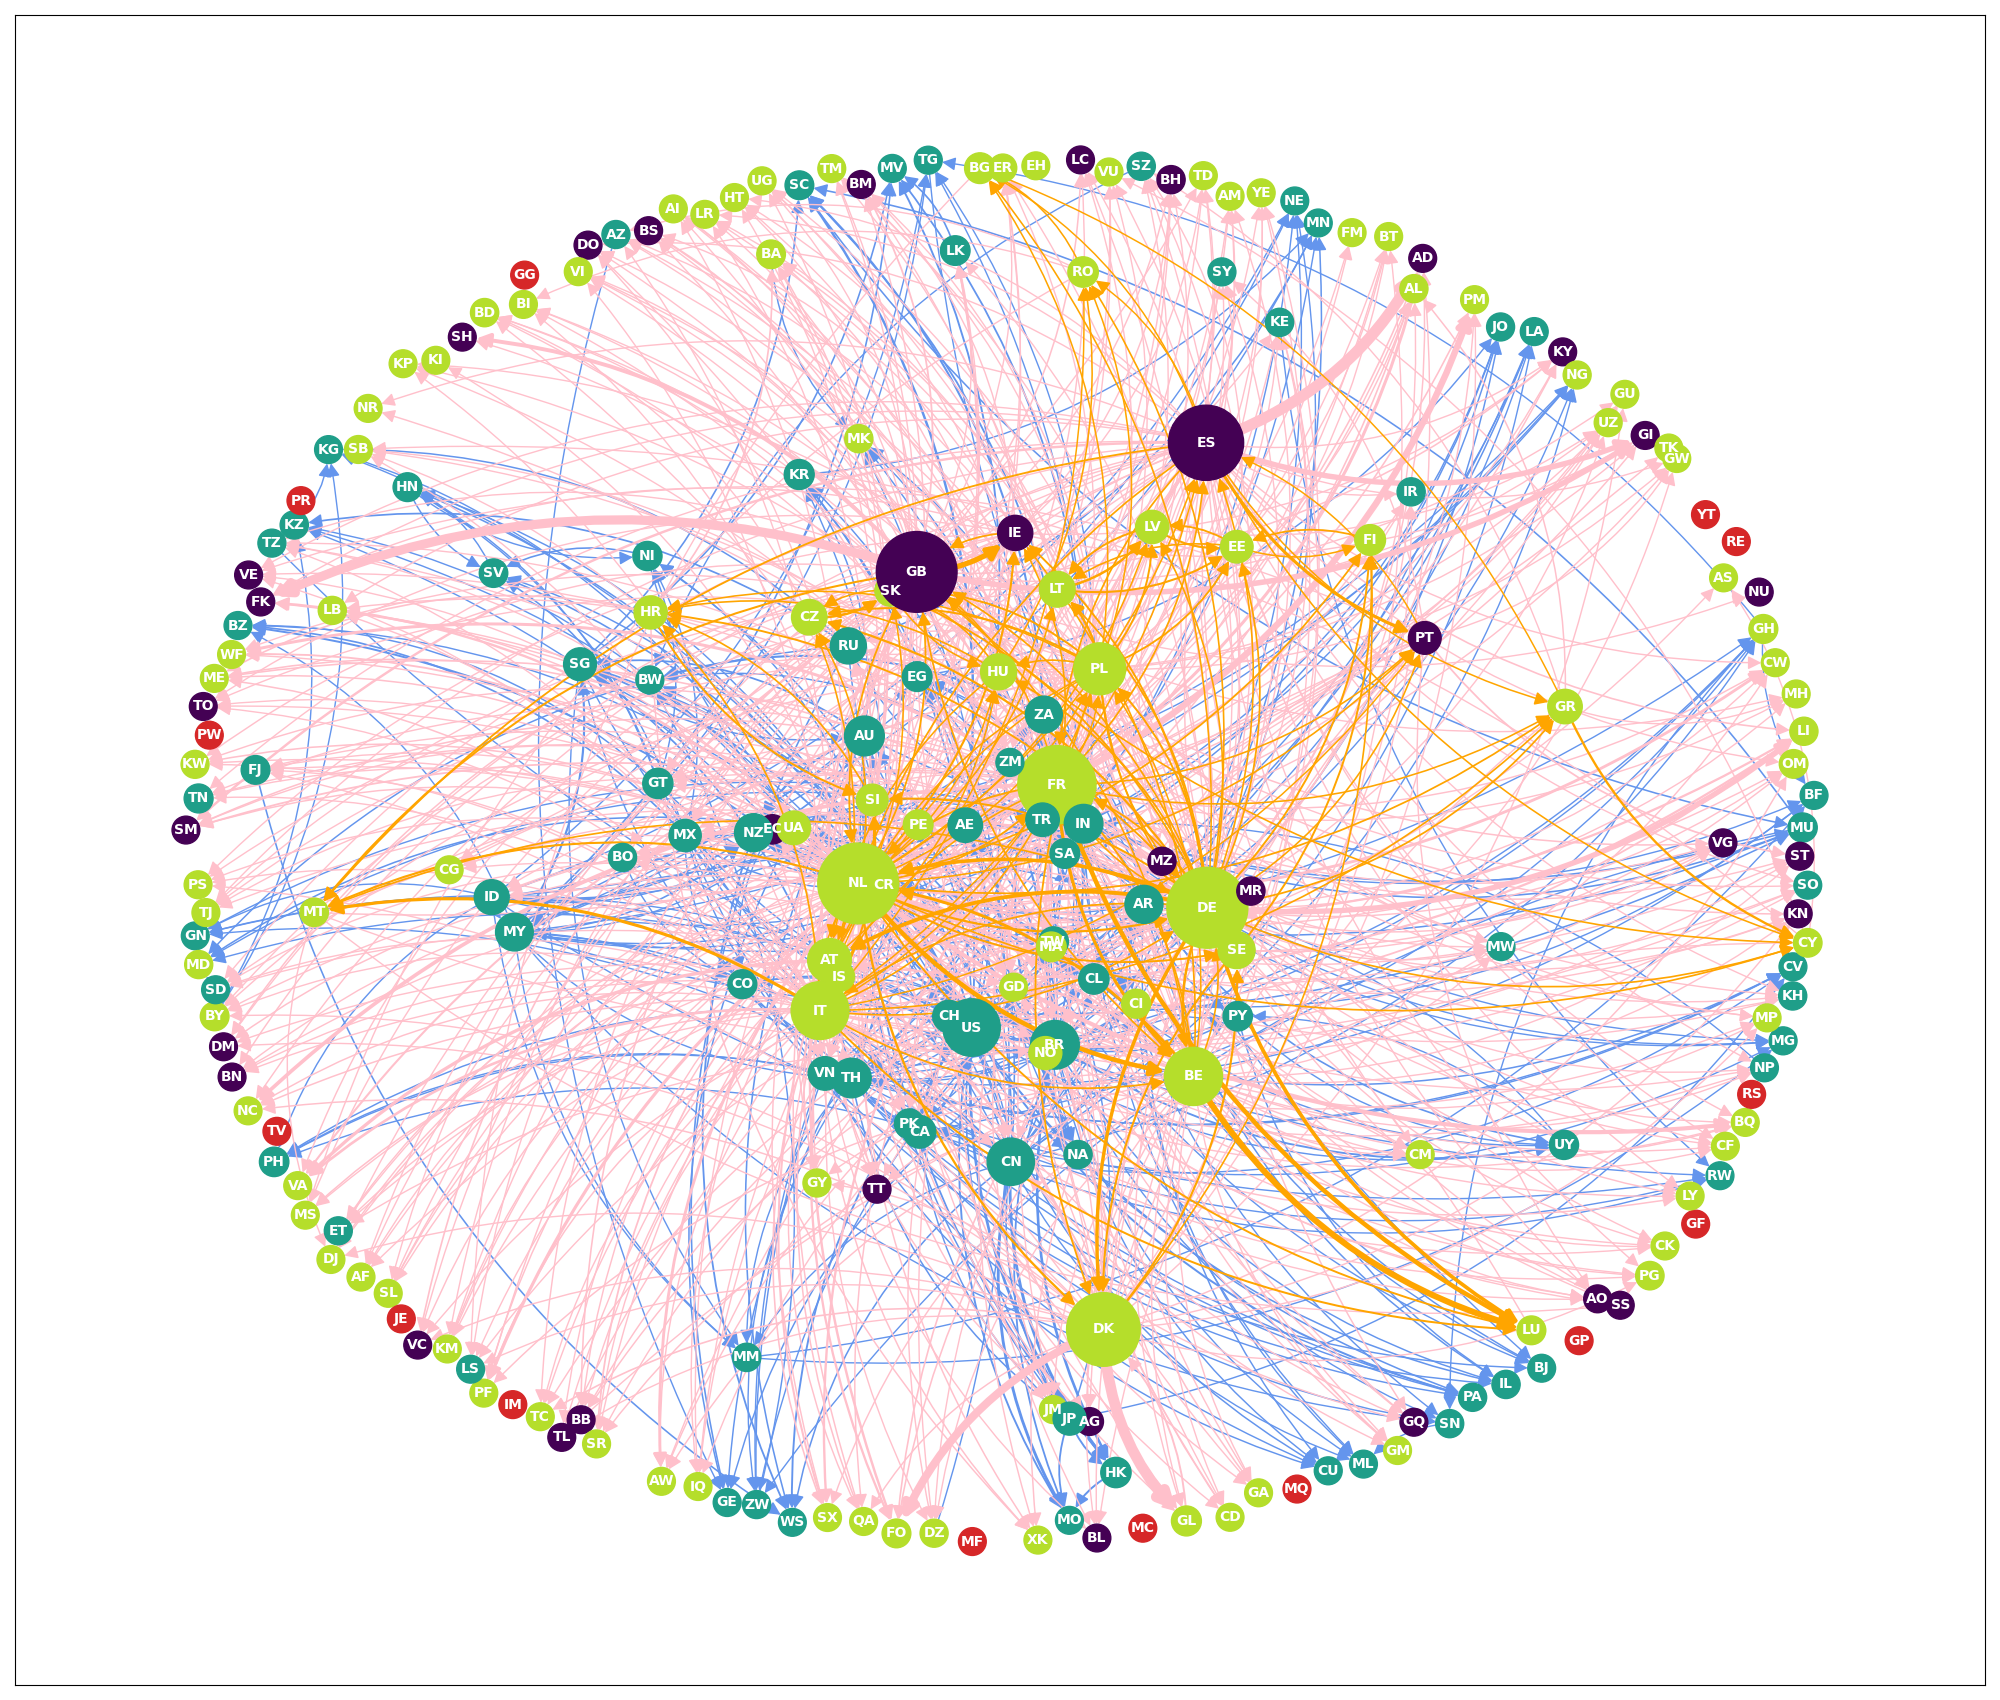
\includegraphics[width=\textwidth]{pics/full_y19_p10_force_144_lou.png}
        \caption{Louvain Method}
        \label{fig:foodnetworklou}
    \end{subfigure}
    \caption[Global trade network of \textit{Food Products} in 2019, with communities.]{Global trade network of \textit{Food Products} in 2019. The size of the node represents the \textit{out-strength} of that country. The color of the node corresponds to the block membership; the color of the edge is \textit{orange} for intra-EU exchanges, \textit{pink} for EU - non-EU exchanges and \textit{azure} for extra-EU exchanges. Only the top 5 import partnership for each country are shown.}
    \label{fig:foodcommunities}
\end{figure}
% GAS AND PETROLEUM
\section{The \textit{Crude Petroleum and Natural Gas} Trade Network}

% - pl nel tempo
% - two strange pl plottati
% 	GAS 2006, in_degree + w
% 	FOOD 2010, in_degree + w
% - network plot
% - nodi fighi
% - ts delle metriche del nodo (pr, degree, weight degree, h/a)
% - plot communities chschshchs (sbm & louv) -> chose year
% - plot network (sbm & louv)

%     1) graph metrics:
%         - over time
%         - power law over time
%     2) node properties:
%         - compared on average tra i nodi
%         - time series of relevant node's + pr
%     3) communities:
%         - grafico schschschschscsch (x2)
%         - plot confronto sbm vs louv 
%             --> fai vedere in cosa sono diversi (perchè le communities rappresentano cose diverse)
%             --> confronto modularities
%         - plot tanti^n plot

The second category that I am going to investigate is \textit{Crude Petroleum and Natural Gas}\footnote{
    From the EU Economic Activity Classification:
    "This division includes the production of crude petroleum, the mining and extraction of oil from oil shale and oil sands and the production of natural gas and recovery of hydrocarbon liquids. This division includes the activities of operating and/or developing oil and gas field properties. Such activities may include drilling, completing and equipping wells; operating separators, emulsion breakers, desalting equipment and field gathering lines for crude petroleum; and all other activities in the preparation of oil and gas up to the point of shipment from the producing property."\cite{eurostat2022website}
}. 
The trade market of Oil and Gas is an essential pillar of international trade, which in 2019 moved around more than XXXX million euros worth of exports. It is the nature of the good itself which makes it a suitable item to be exchanged. In fact, only relatively few countries in the world have access to underground fossil fuel resources, and even less countries have enough of it to be great exporters on the global landscape. According to COMEXT-WTO data, the XXX\% of total global exports of \textit{Crude Petroleum and Natural Gas} were coming from just Y different countries: A,B,C,D,E.
This fact is an indicator of the presence of an oligopoly\footnote{
    An \textit{oligopoly} is a market structure in which a market or industry is dominated by a small number of large sellers or producers. Oligopolies often result from the desire to maximize profits, leading to collusion between companies. This reduces competition, leading to higher prices for consumers and lower wages for employee (from \url{https://en.wikipedia.org/wiki/Oligopoly}).
}, which is a renowned fact in microeconomic research, so that very often it is used as an example of these types of markets \cite{mileva2012oil}.
An oligopolistic structure, however, together with the fact that oil and gas are essential goods for the majority of industrialized modern countries, has the potential to create instability into these countries, should any event disrupt or prevent the full functioning of the trade exchanges. An example of a disruption that had an impact on the global supply chain was the Suez Canal blockage of March 2021 \cite{lee2021suez}, while a more recent event of greater magnitude for the global stability is the Russian invasion of Ukraine of 2022. Earlier this year, on February 24th, Russia crossed the border with Ukraine with military forces: this situation is the result of a long deterioration of the relationships among the two nations and a lengthy streak of violence. It started in 2014 with the Ukrainian revolution and the subsequent detachment of the country from the orbit of pro-Russian nations to institute a pro-western government.
The return of war at the heart of the European continent provoked a shock in the neighboring countries which has had few equals in the history of the community; numerous helps of varying nature have been offered to Ukraine, including financial, humanitarian and also military aid. For this research, the most important aspect is certainly the one concerning the economic sanctions imposed on Russia. In fact, one of the sectors that most drives the Russian economy is that of import-export, especially of natural gas and raw materials to various European countries such as Italy, the Czech Republic and Austria. If, on the one hand, the European Union, considering the close dependence of various countries internally, has imposed significant sanctions on oil, but not on natural gas, on the other hand Russia itself has made several cuts in supplies and raised the prices of this scarce but essential resource \cite{sole2022petrolio,wikipedia2022crisirussia}.
% https://www.ilsole24ore.com/art/petrolio-oro-gas-che-punto-sono-sanzioni-ue-russia-AEyWcbiB
% https://it.wikipedia.org/wiki/Crisi_russo-ucraina
% Il 24 febbraio 2022 la Russia invade l'Ucraina. Questa situazione è stata il risultato di un lungo deterioramento dei rapporti tra i due stati e una lunga successione di violenze, cominciata nel 2014 con la rivoluzione Ucraina e il conseguente distaccamento di quest'ultima dall'orbita degli stati filo-russi per instaurare, invece, un governo filo-occidentale.
% Il ritorno della guerra nel cuore dell'Europa ha provocato uno shock da parte delle altre nazioni che ha avuto pochi eguali nella storia comunitaria; sono stati forniti aiuti di varia natura all'Ucraina, sia dal punto di vista economico, sia dal punto di vista umanitario. Per questo studio, l'aspetto più importante è sicuramente quello che riguarda le sanzioni economiche imposte alla Russia. Infatti, uno dei settori che maggiormente traina l'economia russa è quello dell'import-export, soprattutto di materie prime ai vari paesi Europei come Italia, Repubblica Ceca e Austria.
% Se l'Unione Europea, considerando la stretta dipendenza di vari paesi al proprio interno, ha imposto sanzioni significative sul petrolio, ma non sul gas naturale. La stessa Russia, invece, ha effettuato diversi tagli alle forniture e ha alzato i prezzi di questa risorsa così scarsa ma così essenziale.
Thanks to the availability of data and the tools of network science, we can try to find a reason for why a disruption such as Russia cutting off its gas supply could have such a shaking effect on Europe and the limiting countries. I will follow the same steps as the previous analysis, and thus I will start by having a look at the aggregated metrics of the graph over time. 
In Figure \ref{fig:gasmetrics} we see the time series of the network's \textit{size}, average \textit{degree}, median \textit{page rank} and average \textit{clustering coefficient}. Looking at the upper left plot, we immediately see the effect of the two crises on the trade network size. In the 2008 financial crisis, the amount of trade dropped by more than 10 million euros (per 1000 p.) from one year to the next, while for COVID it even halved in 2020 with respect to 2019. A similar effect can be found in the average degree plot, with the 2020 crisis causing a sudden drop in the mean number of connection of nodes, due to many of these exchanges coming to a halt. Being this market an oligopoly, we may be expecting a higher page rank since a lot of nodes receive incoming edges without having any outgoing, but this is justified by the fact that the exporter nodes which would pass on the page rank to them have a lot of out going links, and thus each of them receives only a small portion of it.

\begin{figure}
    \centering
    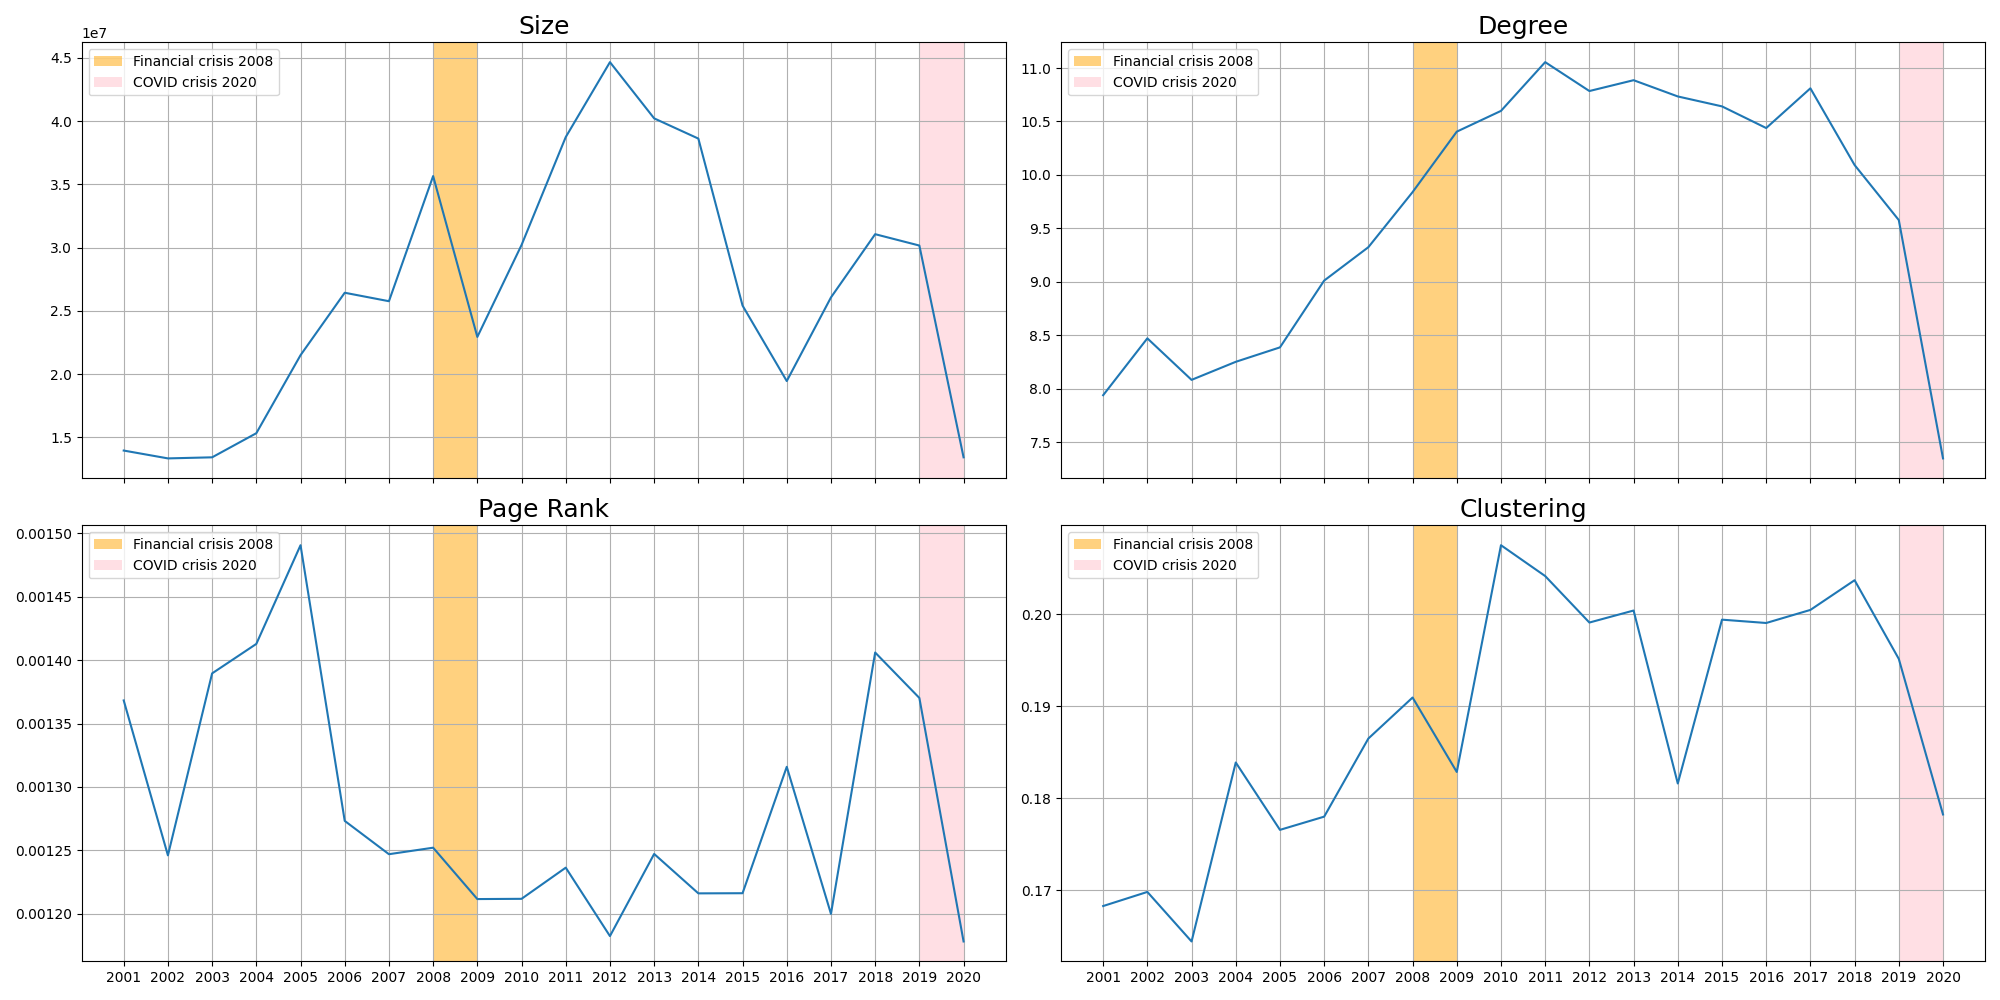
\includegraphics[width=\textwidth]{pics/full_p06_metric_ts.png}
    \caption{Crude petroleum and natural gas Metrics TODO}
    \label{fig:gasmetrics}
\end{figure}

\subsection{Degree distribution}

A secondary query we might try to find an answer to is whether in this trade sector the networks display signs of the \textit{scale-free} property. Hence, we look at Figure \ref{fig:gasdegree}, representing the power law fit over time. Considering the orange lines, indicating the fit of the linear regression in the log-log plot of the degree distribution, which is measured with MAPE, we see that the two weighted metrics are consistently a better fit than the unweighted version. Regarding the values of the \textit{gamma} exponent of the power law, it is similar in all four distributions, oscillating between the values of $0.8$ and $1$. Let us have a look at a specific year, to see whether it is indeed the case of a good power law fit.

\begin{figure}
    \centering
    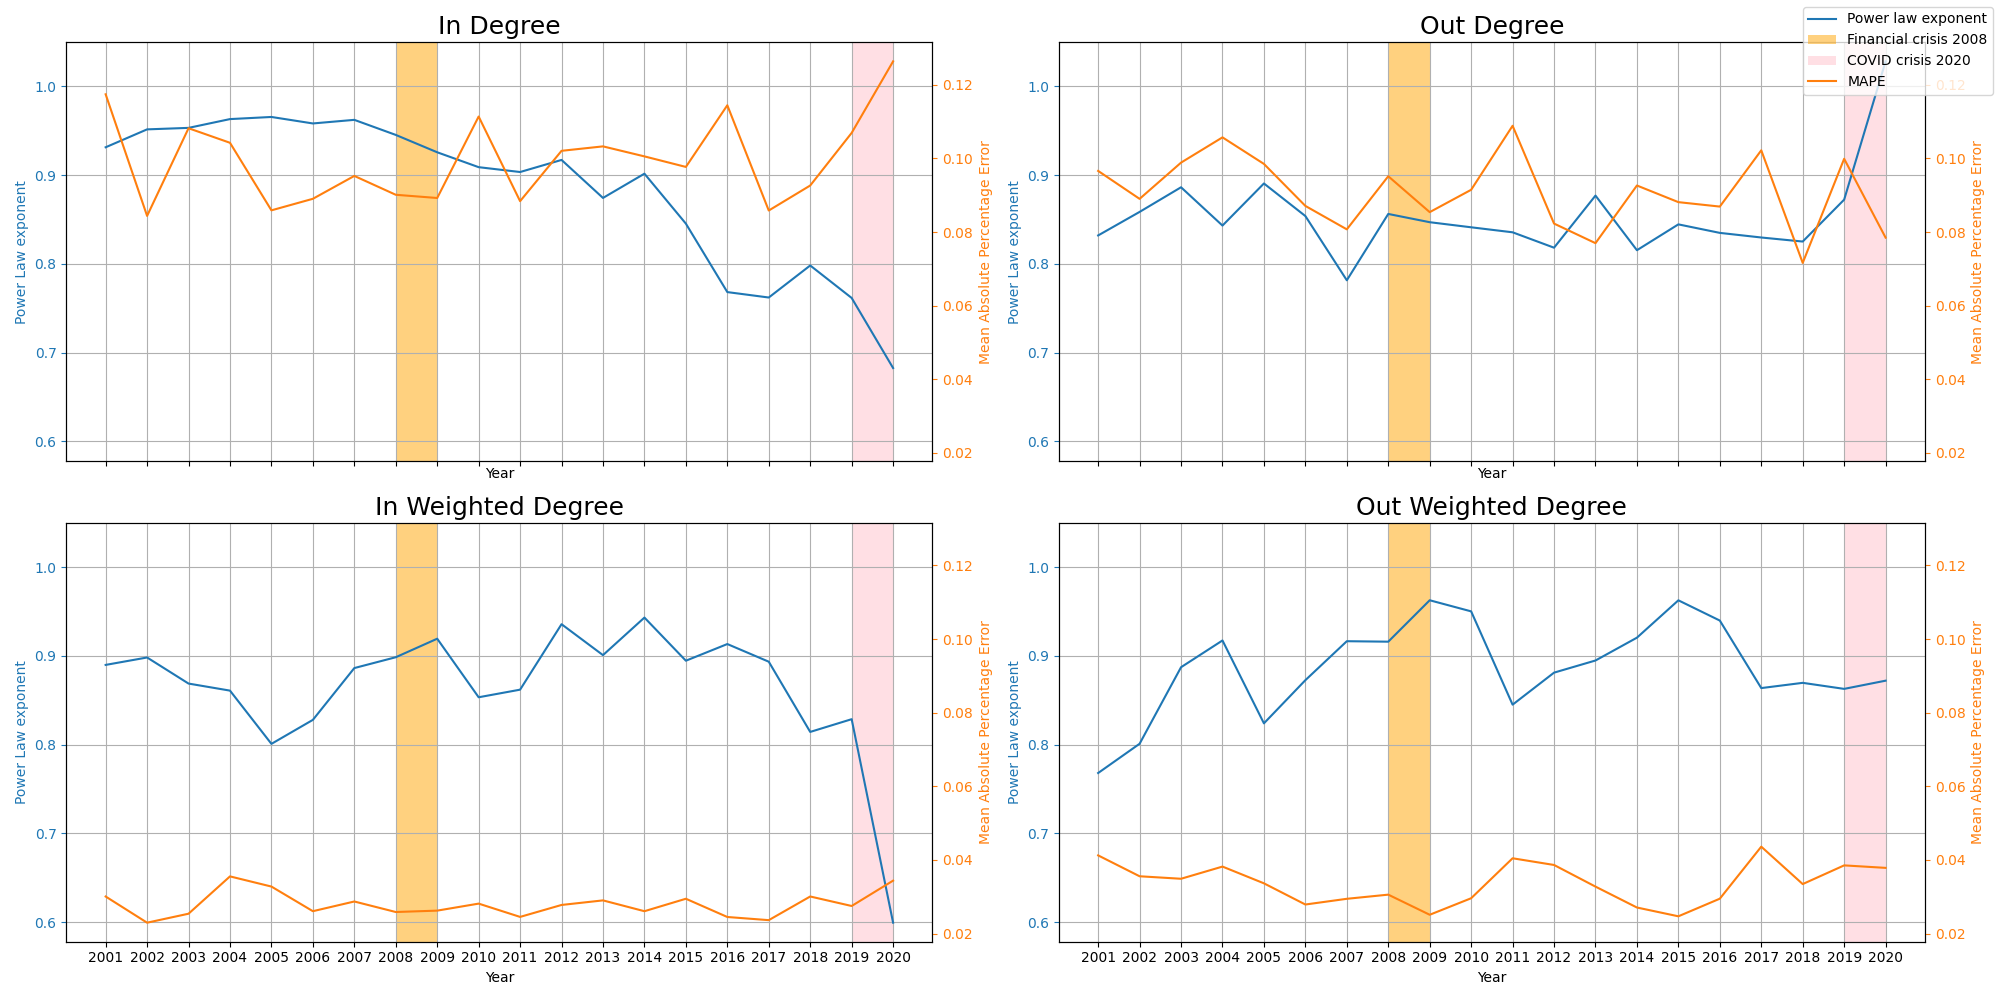
\includegraphics[width=\textwidth]{pics/ts_p06.png}
    \caption{Power law exponents over time of four degree distributions in the \textit{Crude petroleum and natural gas} networks.}
    \label{fig:gasdegree}
\end{figure}

Figure \ref{fig:gasdistrib} displays the degree distribution of the \textit{out degree} and \textit{out weighted degree} of the petroleum and gas trade network in 2010. Both curves seem to be quite fit to the distributions, and in particular the second one, which in fact presents a lower MAPE. The way we can interpret these plots is that the countries which have a high \textit{out degree} are the few oligopolistic exporters of the trade network, while the numerous countries with low degree are those who import from them. The \textit{out weighted degree} distribution is even more unbalanced than the previous one, with very few nodes which have an enormous output of gas and petroleum with respect to a great number of nodes which have no ability to export. By looking even more carefully at the dataset number, we can discover that the isolated point to the bottom right of the plot of the out weight degree is Russia alone, which has in fact a total export normalized value which is three times higher than the second major exporter, Saudi Arabia (although in nominal value they export roughly the same, Russia is known to sell petroleum and gas at a considerably lower price than other countries, thus the output quantity of RU corresponding to that monetary value is huge) \cite{trent2020opec}.
Let us have a look now in the next paragraph at the network plot for the trade of \textit{Crude petroleum and natural gas} in 2010.
% - both quite fit, the second better 
%     1 --- > the countries with high degree are the few exporters
%     2 --- > symptom of small number of countries which are completely dependent on gas from others

\begin{figure}
    \centering
    \begin{subfigure}{\textwidth}
        \centering
        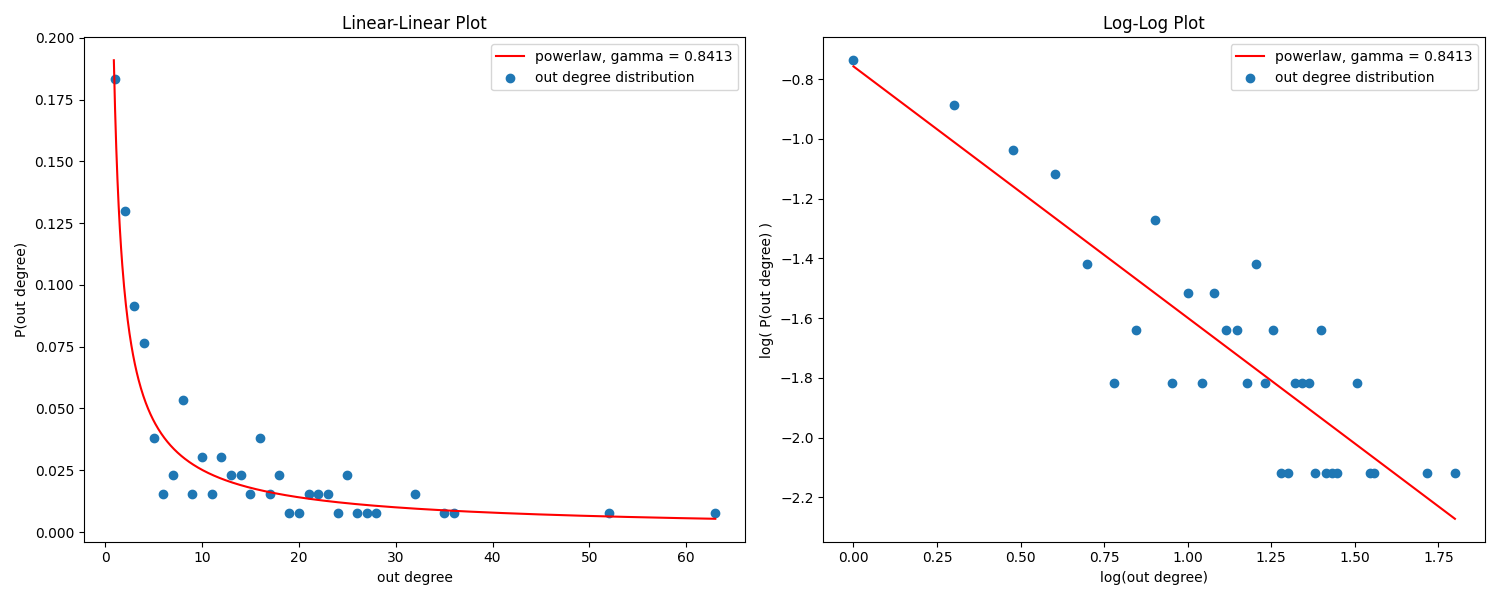
\includegraphics[width=\textwidth]{pics/powerlaw_out_degree_p06_y2010.png}
        \caption{\textit{Out Degree}}
        \label{fig:plgas}
    \end{subfigure}
    
    \begin{subfigure}{\textwidth}
        \centering
        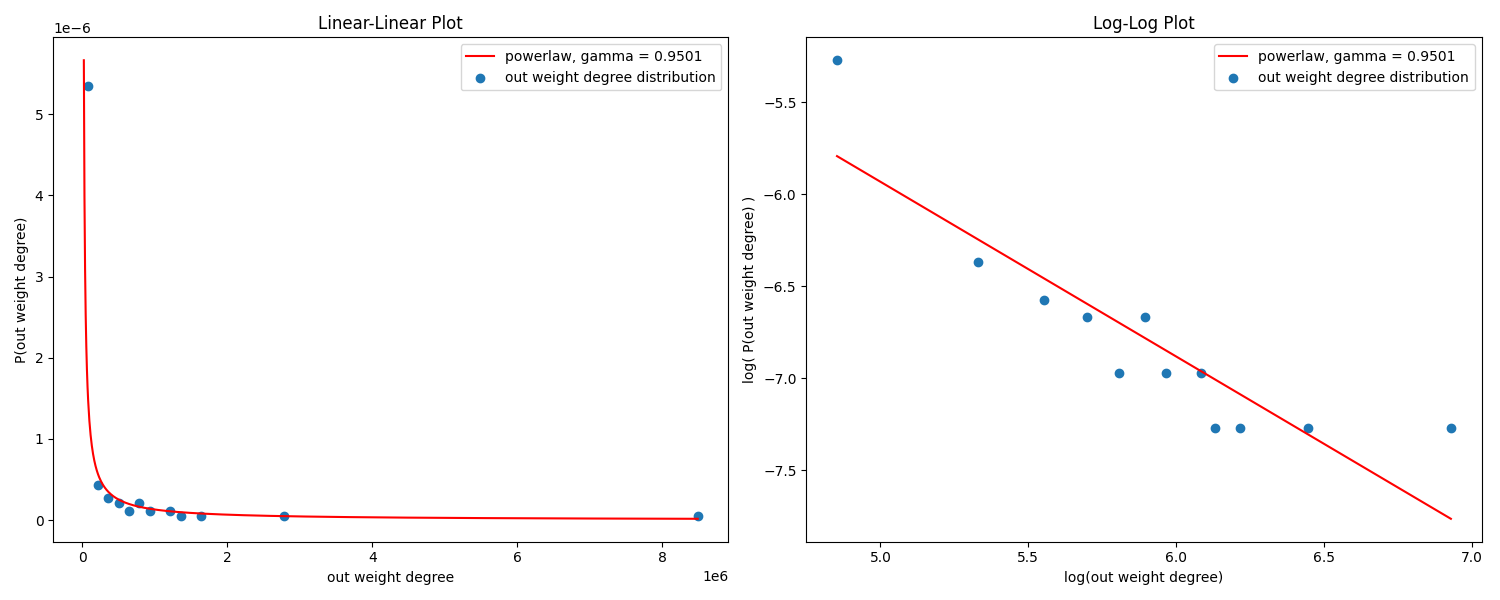
\includegraphics[width=\textwidth]{pics/powerlaw_out_weight_degree_p06_y2010.png}
        \caption{\textit{Out Weighted Degree}}
        \label{fig:plgasw}
    \end{subfigure}
    \caption{\textit{Crude petroleum and natural gas} trade network's degree distribution in 2010, with power law fit.}
    \label{fig:gasdistrib}
\end{figure}


\subsection{Network plot and node properties}

The plot in Figure \ref{fig:gasnetwork} of the petroleum and gas network is represented with the force-directed layout, which permits us to comment on the position of countries in the network. Indeed, we find positioned in the middle of the graph, countries which are the major global players in this market, and they are linked through a dense web of exchanges with other countries: they are Russia (RU), Saudi Arabia (SA), Arab Emirates (AE), Qatar (QA) and Norway (NO). The size of the node itself indicates the total output, and as it was mentioned above, Russia is by far the biggest in terms of normalized output. From there, a lot of thick edges (indicating heavier links) origin and go towards EU countries (\textit{pink} edges) or non-EU (\textit{azure} edges). A notable difference with the network of \textit{Food Products} is that in this case, many EU countries (indicated in \textit{blue}) become peripheral countries, which only receive imports of gas and don't produce any for export. There are a few EU countries in the middle which often act as redistributors, such as the Netherlands (NL), France (FR) and the United Kingdom (GB): they receive imports from other central countries and then export part of it to their neighboring ones. An additional characteristic that we can notice in the plot is a thick web of azure exchanges in the lower part of the network, surrounding the countries of SA, QA, AE. This represents the trade of petroleum and gas which originates from Middle East countries, and the receiving ends of those edges are countries which depend on such producers: in particular, among the highest importers of these good there are the United States (US), Japan (JP) and China (CN), all of which have an \textit{in degree} of more than 30 (in the case of China it is 53, which the highest among world countries).


\begin{figure}
    \centering
    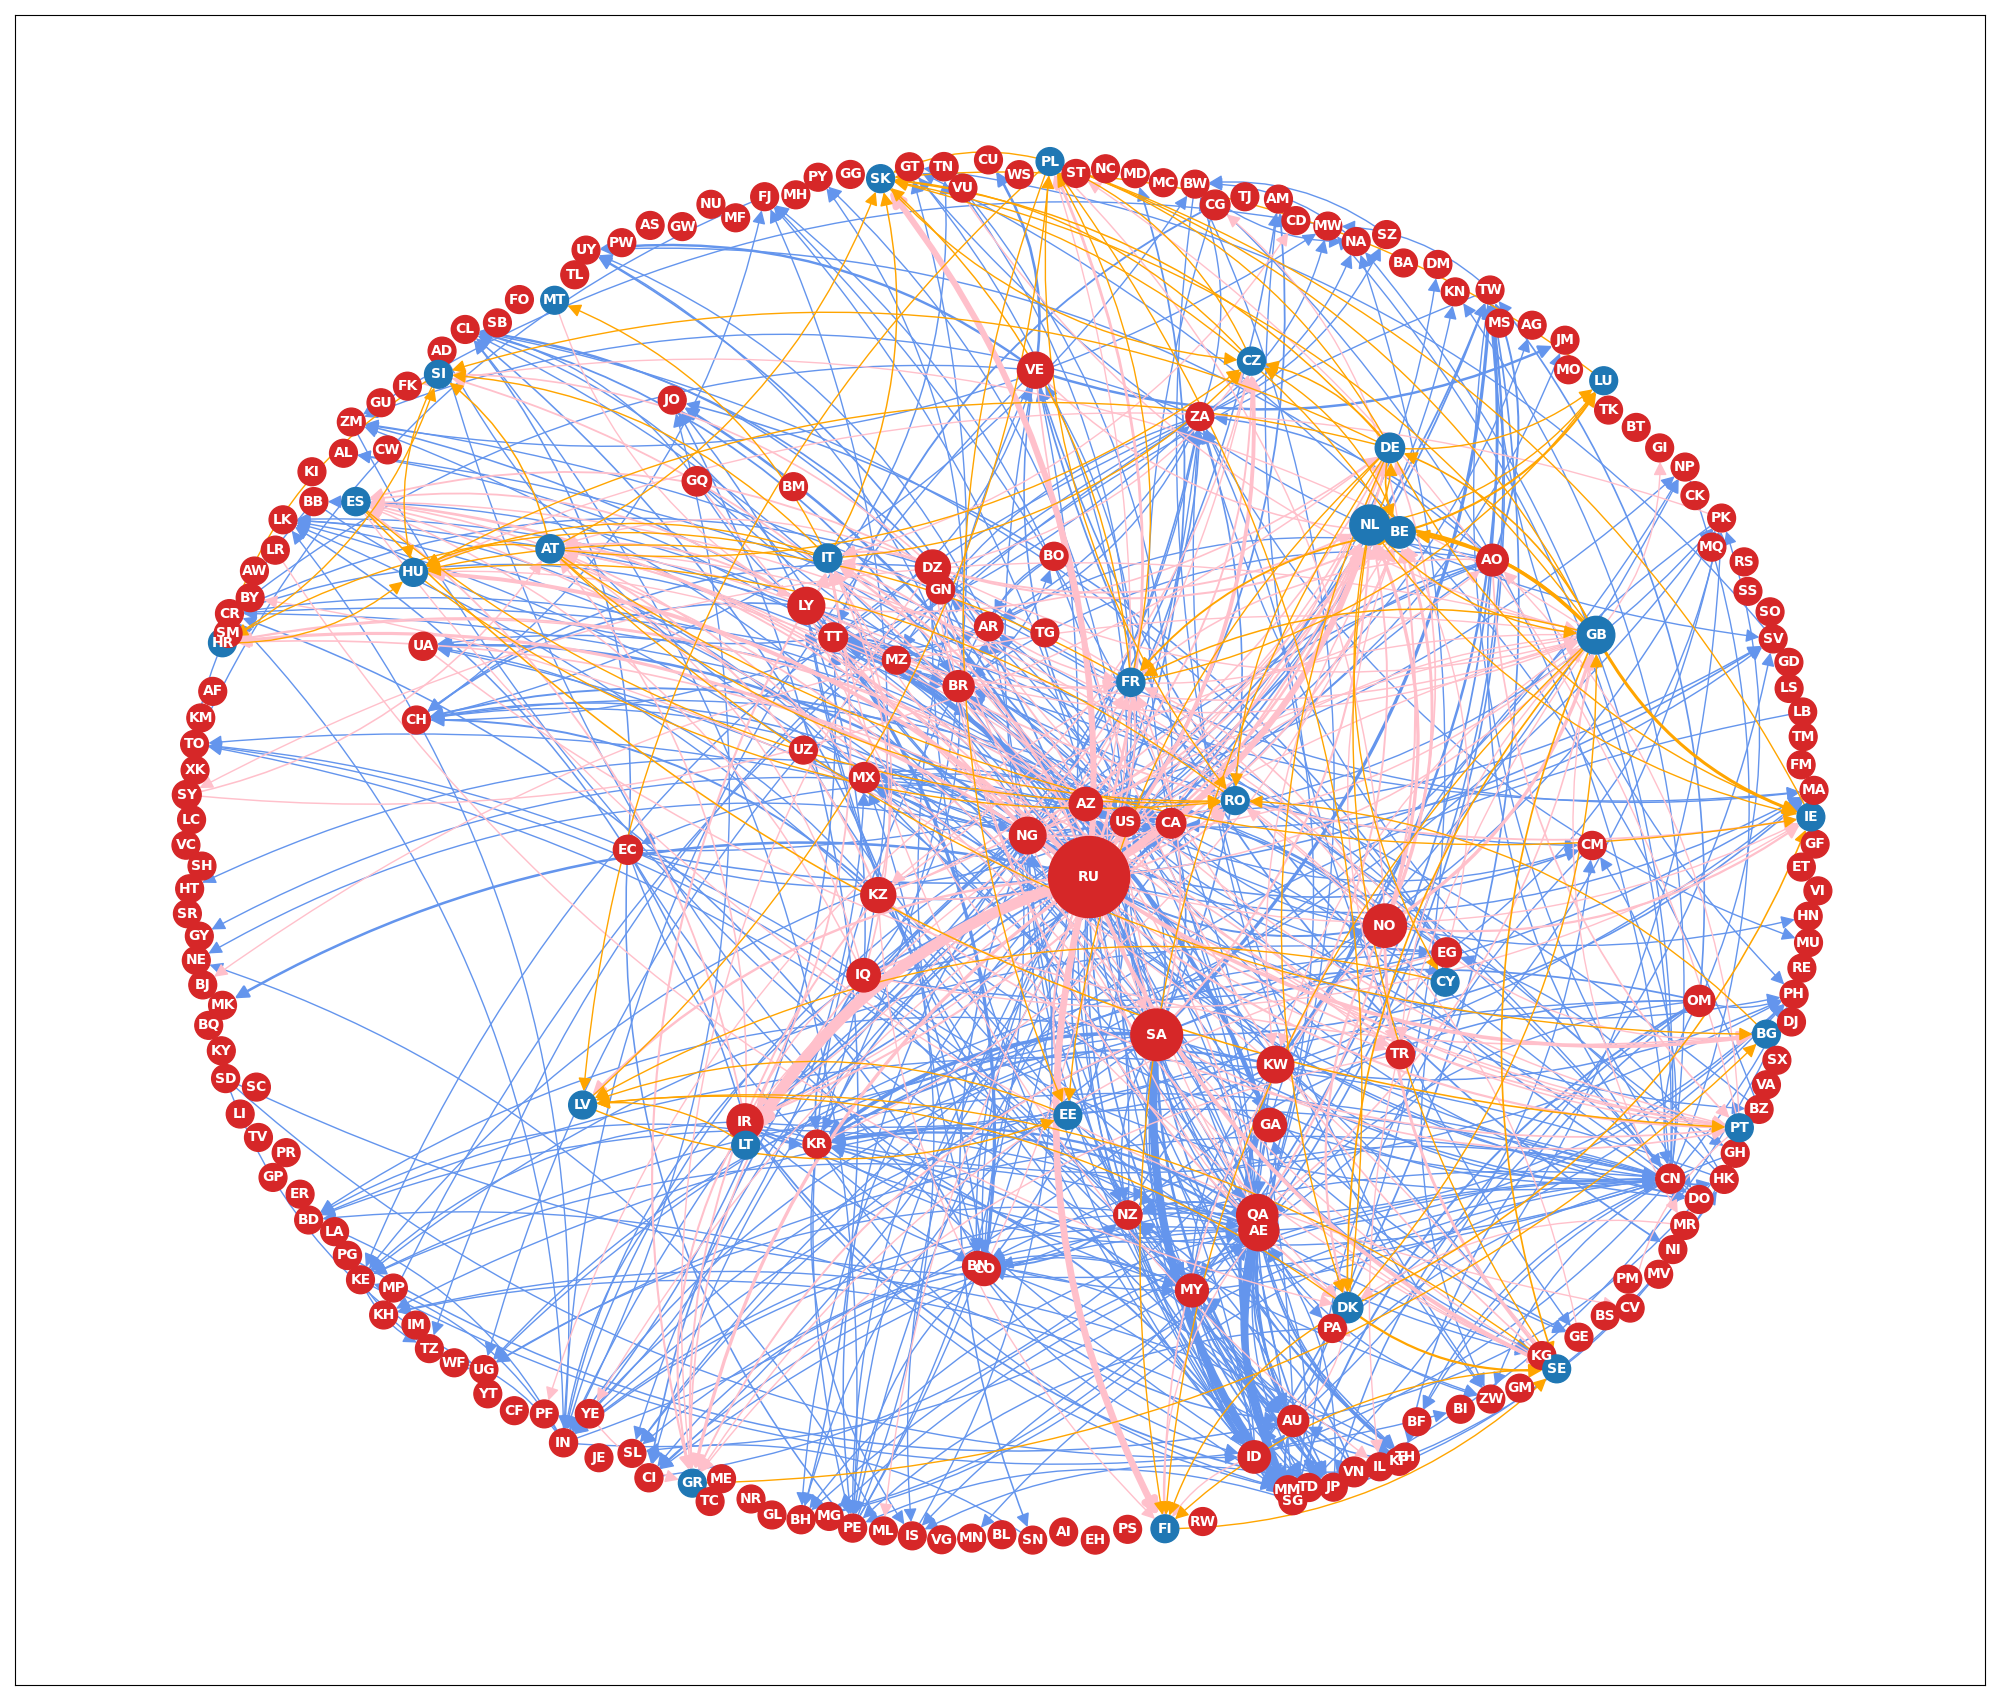
\includegraphics[width=\textwidth]{pics/full_y10_p06_force_120.png}
    \caption[Global trade network of \textit{Crude petroleum and natural gas} in 2010.]{Global trade network of \textit{Crude petroleum and natural gas} in 2010. The size of the node represents the \textit{out-strength} of that country. The color of the node indicates EU countries (\textit{blue}) and non-EU (\textit{red}); the color of the edge is \textit{orange} for intra-EU exchanges, \textit{pink} for EU - non-EU exchanges and \textit{azure} for extra-EU exchanges. Only the top 5 import partnership for each country are shown.}
    \label{fig:gasnetwork}
\end{figure}

Nevertheless, the high count of import partnerships of these countries is a valuable strategy in assuring continuous supply of this good, and in fact they don't appear on the top list of highest dependencies on petroleum and gas supplies, neither in 2010, nor more recently in 2019 (which is shown in \cref{tab:top10gasimp}). The numbers in this table provide evidence in support of the claim that countries, especially European ones, depend on Russian imports. Five out of ten exports of this table are links from Russia to countries such as Lithuania (LT), Finland (FI) and the Netherlands (NL), and we see that the situation has remained stable also in 2019. 
For what it concerns Italy, instead, we observe a change in behavior over the course of nine years. Figuring at the top of imports of \textit{Crude petroleum and natural gas} in 2010 there were Libya (LY), Russia (RU) and Algeria (DZ), at around similar levels. The situation has changed in 2019, where only Russia has maintained its status as leading supplier for Italy, whereas Libya and Algeria basically halved their exports in terms of normalized values. A possible cause of this may have been the Libyan crisis of 2011, linked with the riots and protests across all Middle Eastern and North African countries, known as the "Arab Spring" \cite{wikipedia2011libia}.

\begin{table}
    \centering
    % \resizebox{0.45\textwidth}{!}{
    \resizebox{0.3\textwidth}{!}{
\begin{subtable}{0.3\textwidth}
    \centering
    \begin{tabular}{llr}
    \toprule
    Country From & Country To & Value €/1000 p. \\
    \midrule
              RU &         LT &      1559671.18 \\
              NL &         BE &      1182214.94 \\
              SA &         SG &      1072159.63 \\
              RU &         FI &       862697.08 \\
              RU &         NL &       794297.04 \\
              QA &         SG &       760397.50 \\
              RU &         SK &       757951.78 \\
              AE &         SG &       578737.40 \\
              GA &         TT &       447159.96 \\
              RU &         SE &       415147.96 \\
    \midrule
              LY &         IT &       179972.18 \\
              RU &         IT &       163684.12 \\
              DZ &         IT &       124351.88 \\
              AZ &         IT &        88476.04 \\
              IR &         IT &        73648.57 \\
              IQ &         IT &        52013.73 \\
              SA &         IT &        40190.73 \\
              KZ &         IT &        34114.82 \\
              QA &         IT &        24683.36 \\
              NO &         IT &        20077.77 \\
    \bottomrule
    \end{tabular}
    \caption{Year 2010}
    \label{tab:top10gasimport2010}
\end{subtable}
}
\hfill
\resizebox{0.3\textwidth}{!}{
\begin{subtable}{0.3\textwidth}
    \centering
    \begin{tabular}{llr}
    \toprule
    Country From & Country To & Value €/1000 p. \\
    \midrule
              NL &         BE &      1137264.82 \\
              RU &         LT &      1132888.14 \\
              AE &         SG &      1008058.09 \\
              GB &         GI &       975584.21 \\
              RU &         FI &       822037.96 \\
              QA &         SG &       678777.87 \\
              RU &         NL &       659501.86 \\
              RU &         SK &       496666.08 \\
              SA &         SG &       449912.07 \\
              ID &         SG &       438746.74 \\
    \midrule
              RU &         IT &       160747.70 \\
              AZ &         IT &        80488.00 \\
              IQ &         IT &        79245.86 \\
              LY &         IT &        73654.21 \\
              DZ &         IT &        60418.95 \\
              SA &         IT &        34539.17 \\
              KZ &         IT &        30295.88 \\
              NG &         IT &        23981.59 \\
              QA &         IT &        19787.63 \\
              US &         IT &        13775.67 \\
    \bottomrule
    \end{tabular}
    \caption{Year 2019}
    \label{tab:top10gasimport2019}
\end{subtable}
}
    % }
    \caption{Top 10 edges by weight in the \textit{Crude petroleum and natural gas} market and top 10 incoming edges for IT by weight, in 2019.}
    \label{tab:top10gasimp}
\end{table}

Given the central role that has Russia in this particular market, let us have a look at the single node's metrics and how they evolved in time, which might give us insights into the role of Russia in this trade market over the last 20 years. In \cref{fig:rusmetrics}, there are displayed six relevant metrics for the node centrality. It is interesting to see that the values of Page Rank and Authority are essentially constant at zero: this is not surprising since the role of Russia as one of the biggest world exporters implies that it has many edges which point towards other nodes, thus distributing the page rank. At the same time, there are basically no incoming edges for Russia, and this explains the Authority Value. On the contrary, having a high number of outgoing edges is what drives up the Hub value of RU. According to these plots, we could say that Russia had a peak of importance in the market in the three years of 2010-2012, as it can be derived from the high values of Hub, Out Degree and Out Weighted Degree. This is in line with the reported news that one can find on that period \cite{reutersru1,reutersru2}.

\begin{figure}
    \centering
    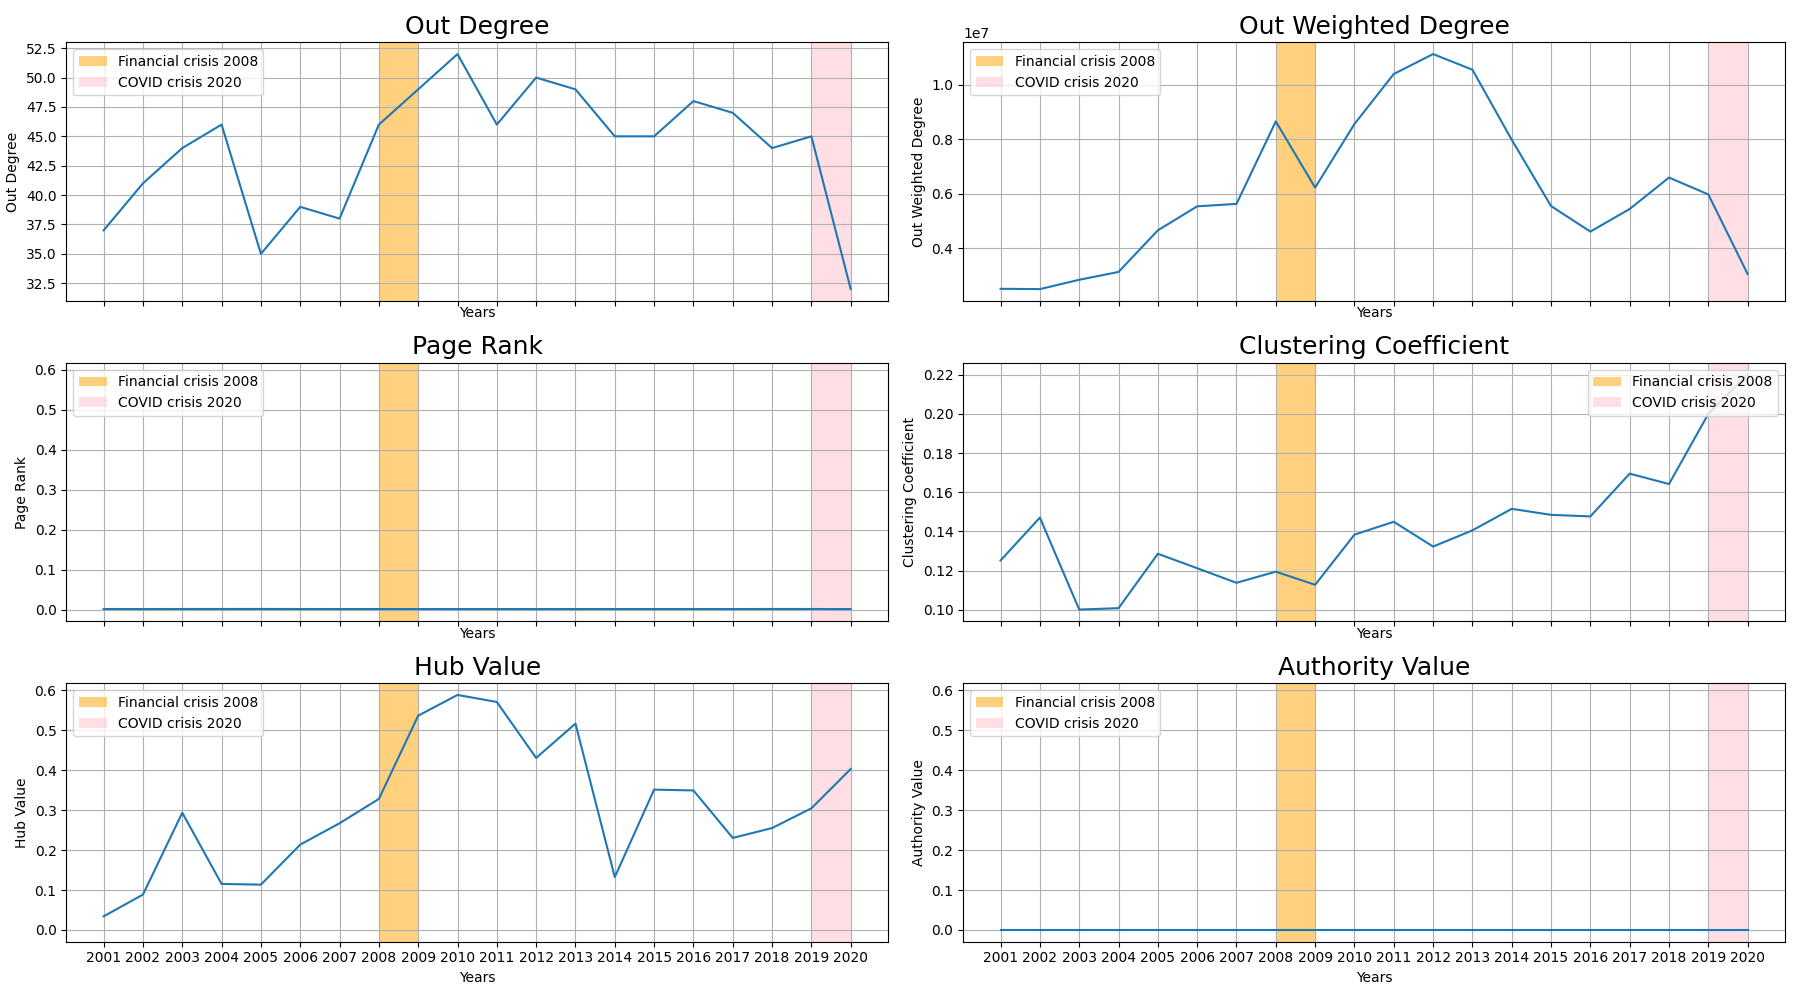
\includegraphics[width=\textwidth]{pics/RU_p06_metric_ts.png}
    \caption{Network metrics for Russia (RU) of the trade market of \textit{Crude petroleum and natural gas} over the years.}
    \label{fig:rusmetrics}
\end{figure}


\subsection{Community detection}

As it was done for the previous category, we can explore the outcomes of the algorithms for community detection (DCSBM and Louvain), in order to search for clusters of countries trading intensely or to see whether these present evidences of a core-periphery structure. Let us start by looking at the parallel categories plot of \cref{fig:commgas}. In this market sector, the Degree Corrected SBM has identified three communities in 2019 (\cref{fig:dcgas}), one of which, the yellow one (3), seems to have been defined since the first years. At the same time, also the output of the Louvain method (\cref{fig:lougas}) in 2019 is composed of three main communities, with two small additional ones. Given this results, it is of interest to understand whether the two algorithms have returned similar block memberships, that is to say whether the communities refer to the same set of nodes. The communities are plotted in \cref{fig:gascommunities}, once for each method. If we consider the first figure, we start by noticing that Russia (RU) has a different color than the Middle Eastern competitor countries, which instead belong to the green community. Therefore, we can conclude that the cluster of countries in purple (1) is made of those countries which have strong import partnerships with Russia (including Italy), while the cluster in green (2) comprises nodes which trade considerably with Saudi Arabia (SA), Arab Emirates (AE), Qatar (QA) and others. A similar community structure can be found in the second plot, from the Louvain method: here the cluster of nodes orbiting Russia is in green (3), while the Middle Eastern block is in blue (2). However, a relevant difference with DCSBM that we can observe here is the following: while in the previous plot the third community includes those nodes which are at the periphery of the network and don't have a relevant role in this trade market, in the second plot we see the third community at the center of the network, made of nodes such as the United States (US), Norway (NO), Canada (CA), the Netherlands (NL) and the United Kingdom (GB).

\begin{figure}
    \centering
    \begin{subfigure}{\textwidth}
        \centering
        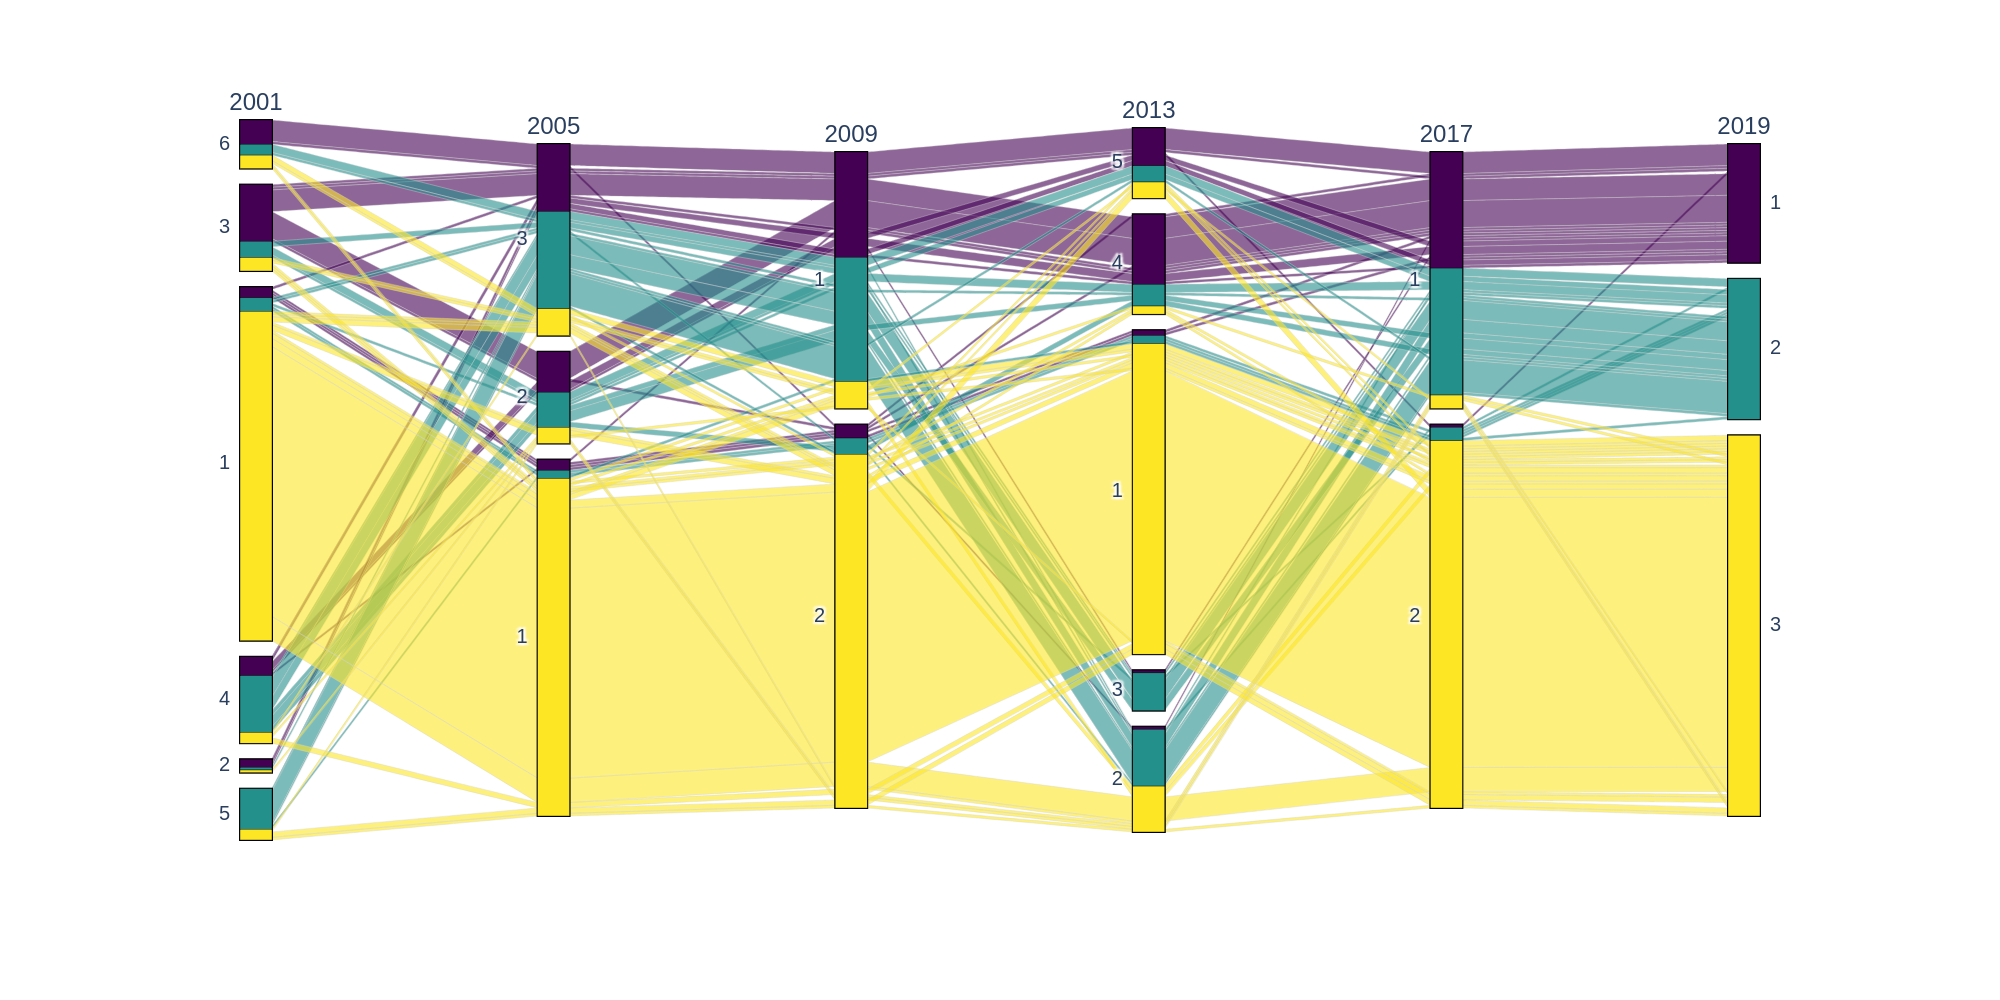
\includegraphics[width=\textwidth]{pics/dc_p06.png}
        \caption{Degree Corrected SBM}
        \label{fig:dcgas}
    \end{subfigure}
    \begin{subfigure}{\textwidth}
        \centering
        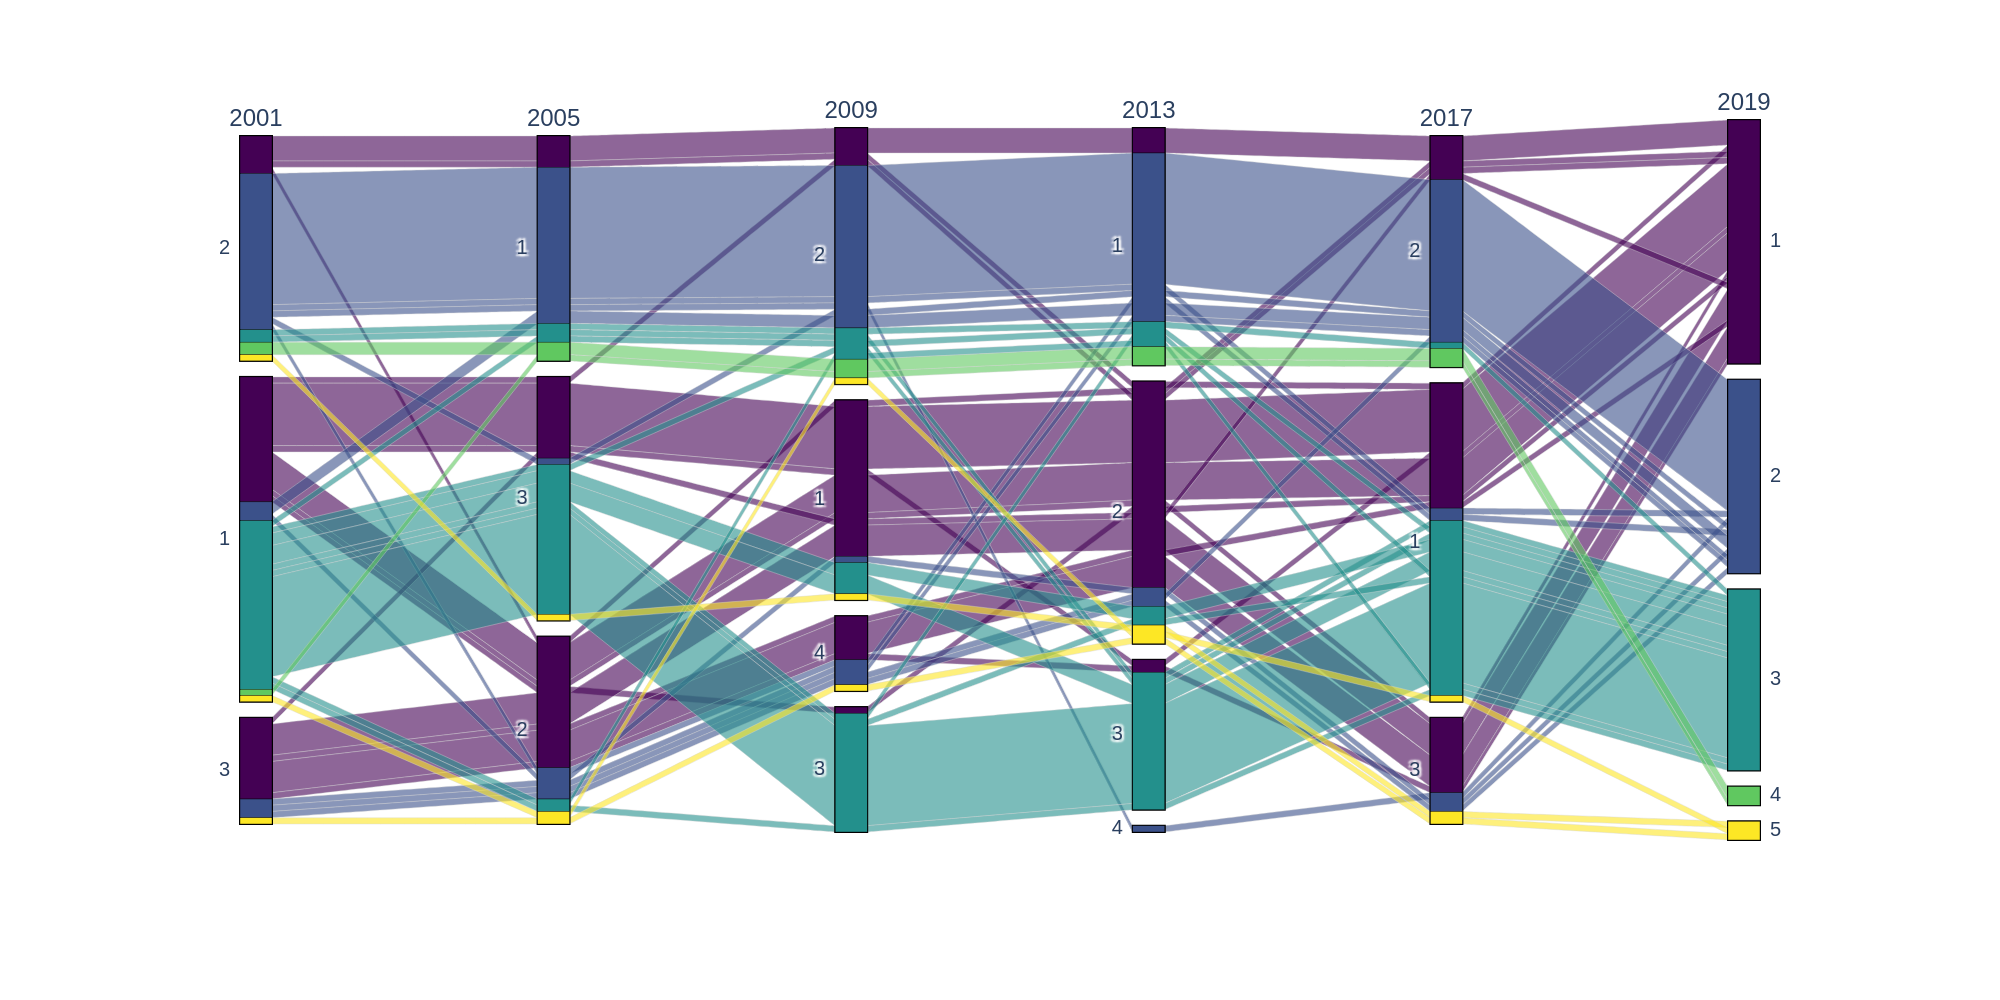
\includegraphics[width=\textwidth]{pics/lou_p06.png}
        \caption{Louvain Method}
        \label{fig:lougas}
    \end{subfigure}
    \caption[Evolution over time of the communities of the \textit{Crude petroleum and natural gas} trade network.]{Evolution over time of the communities of the \textit{Crude petroleum and natural gas} trade network. Communities are shown every 4 years, plus 2019. The colors refer to the memberships in 2019.}
    \label{fig:commgas}
\end{figure}


\begin{figure}
    \centering
    \begin{subfigure}{0.5\textheight}
        \centering
        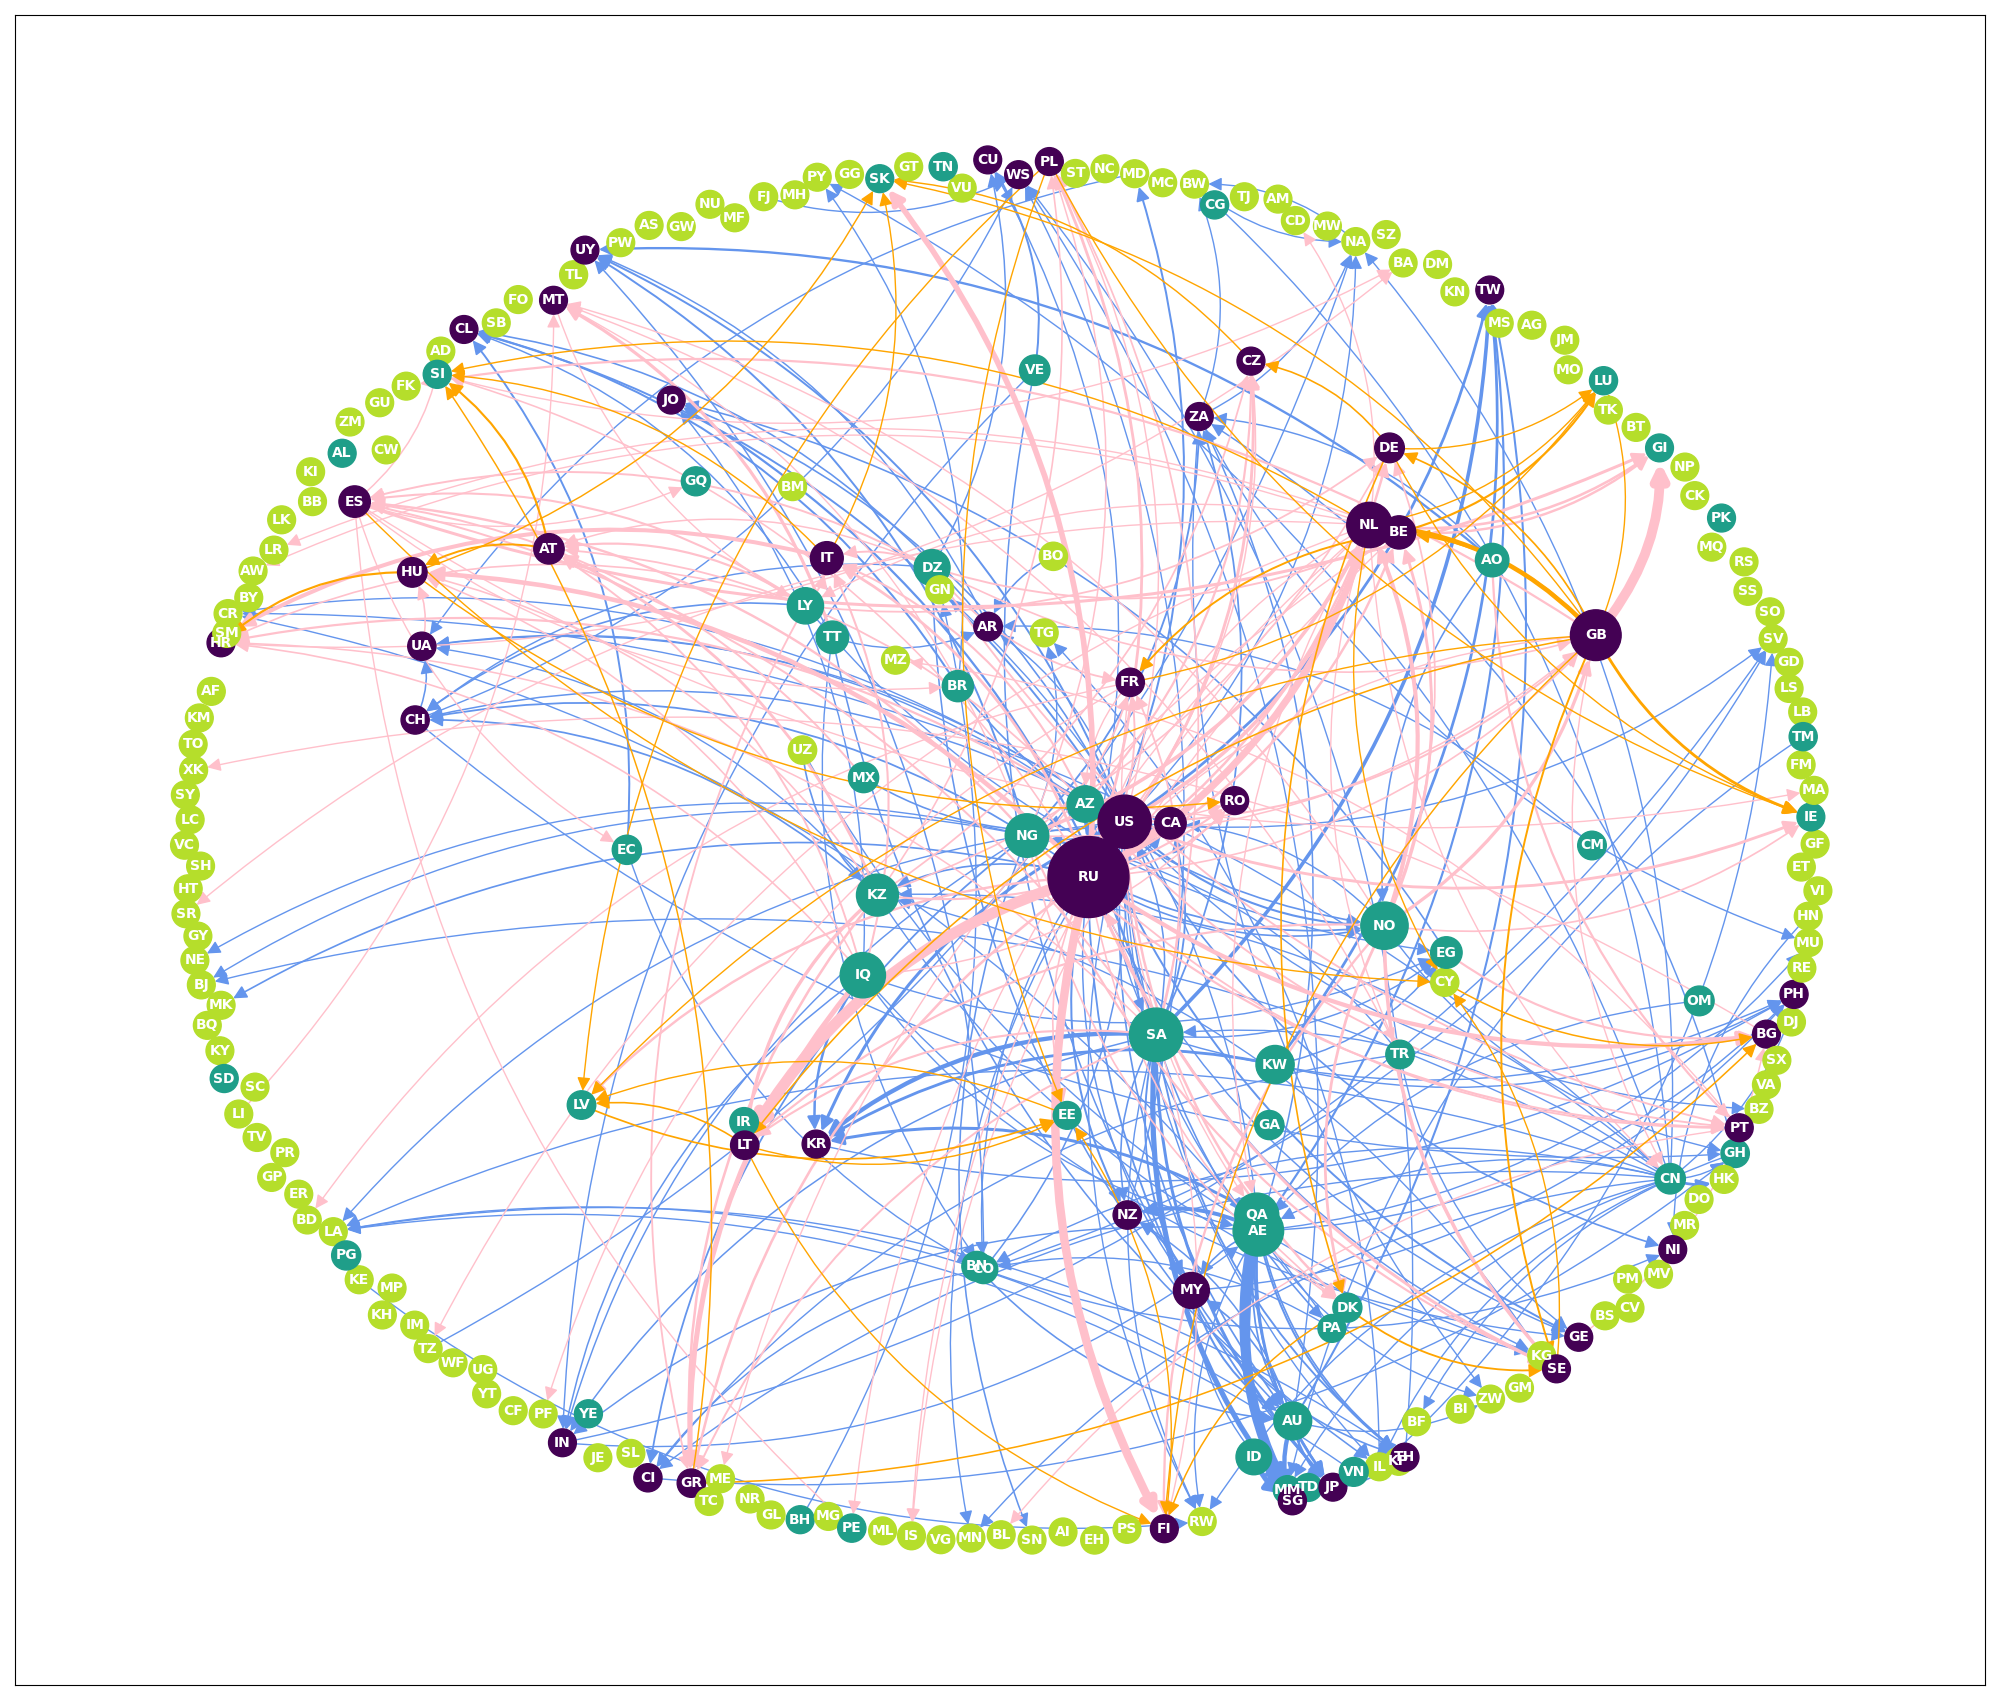
\includegraphics[width=\textwidth]{pics/full_y19_p06_force_146_dc.png}
        \caption{Degree Corrected SBM}
        \label{fig:gasnetworkdc}
    \end{subfigure}

    \begin{subfigure}{0.5\textheight}
        \centering
        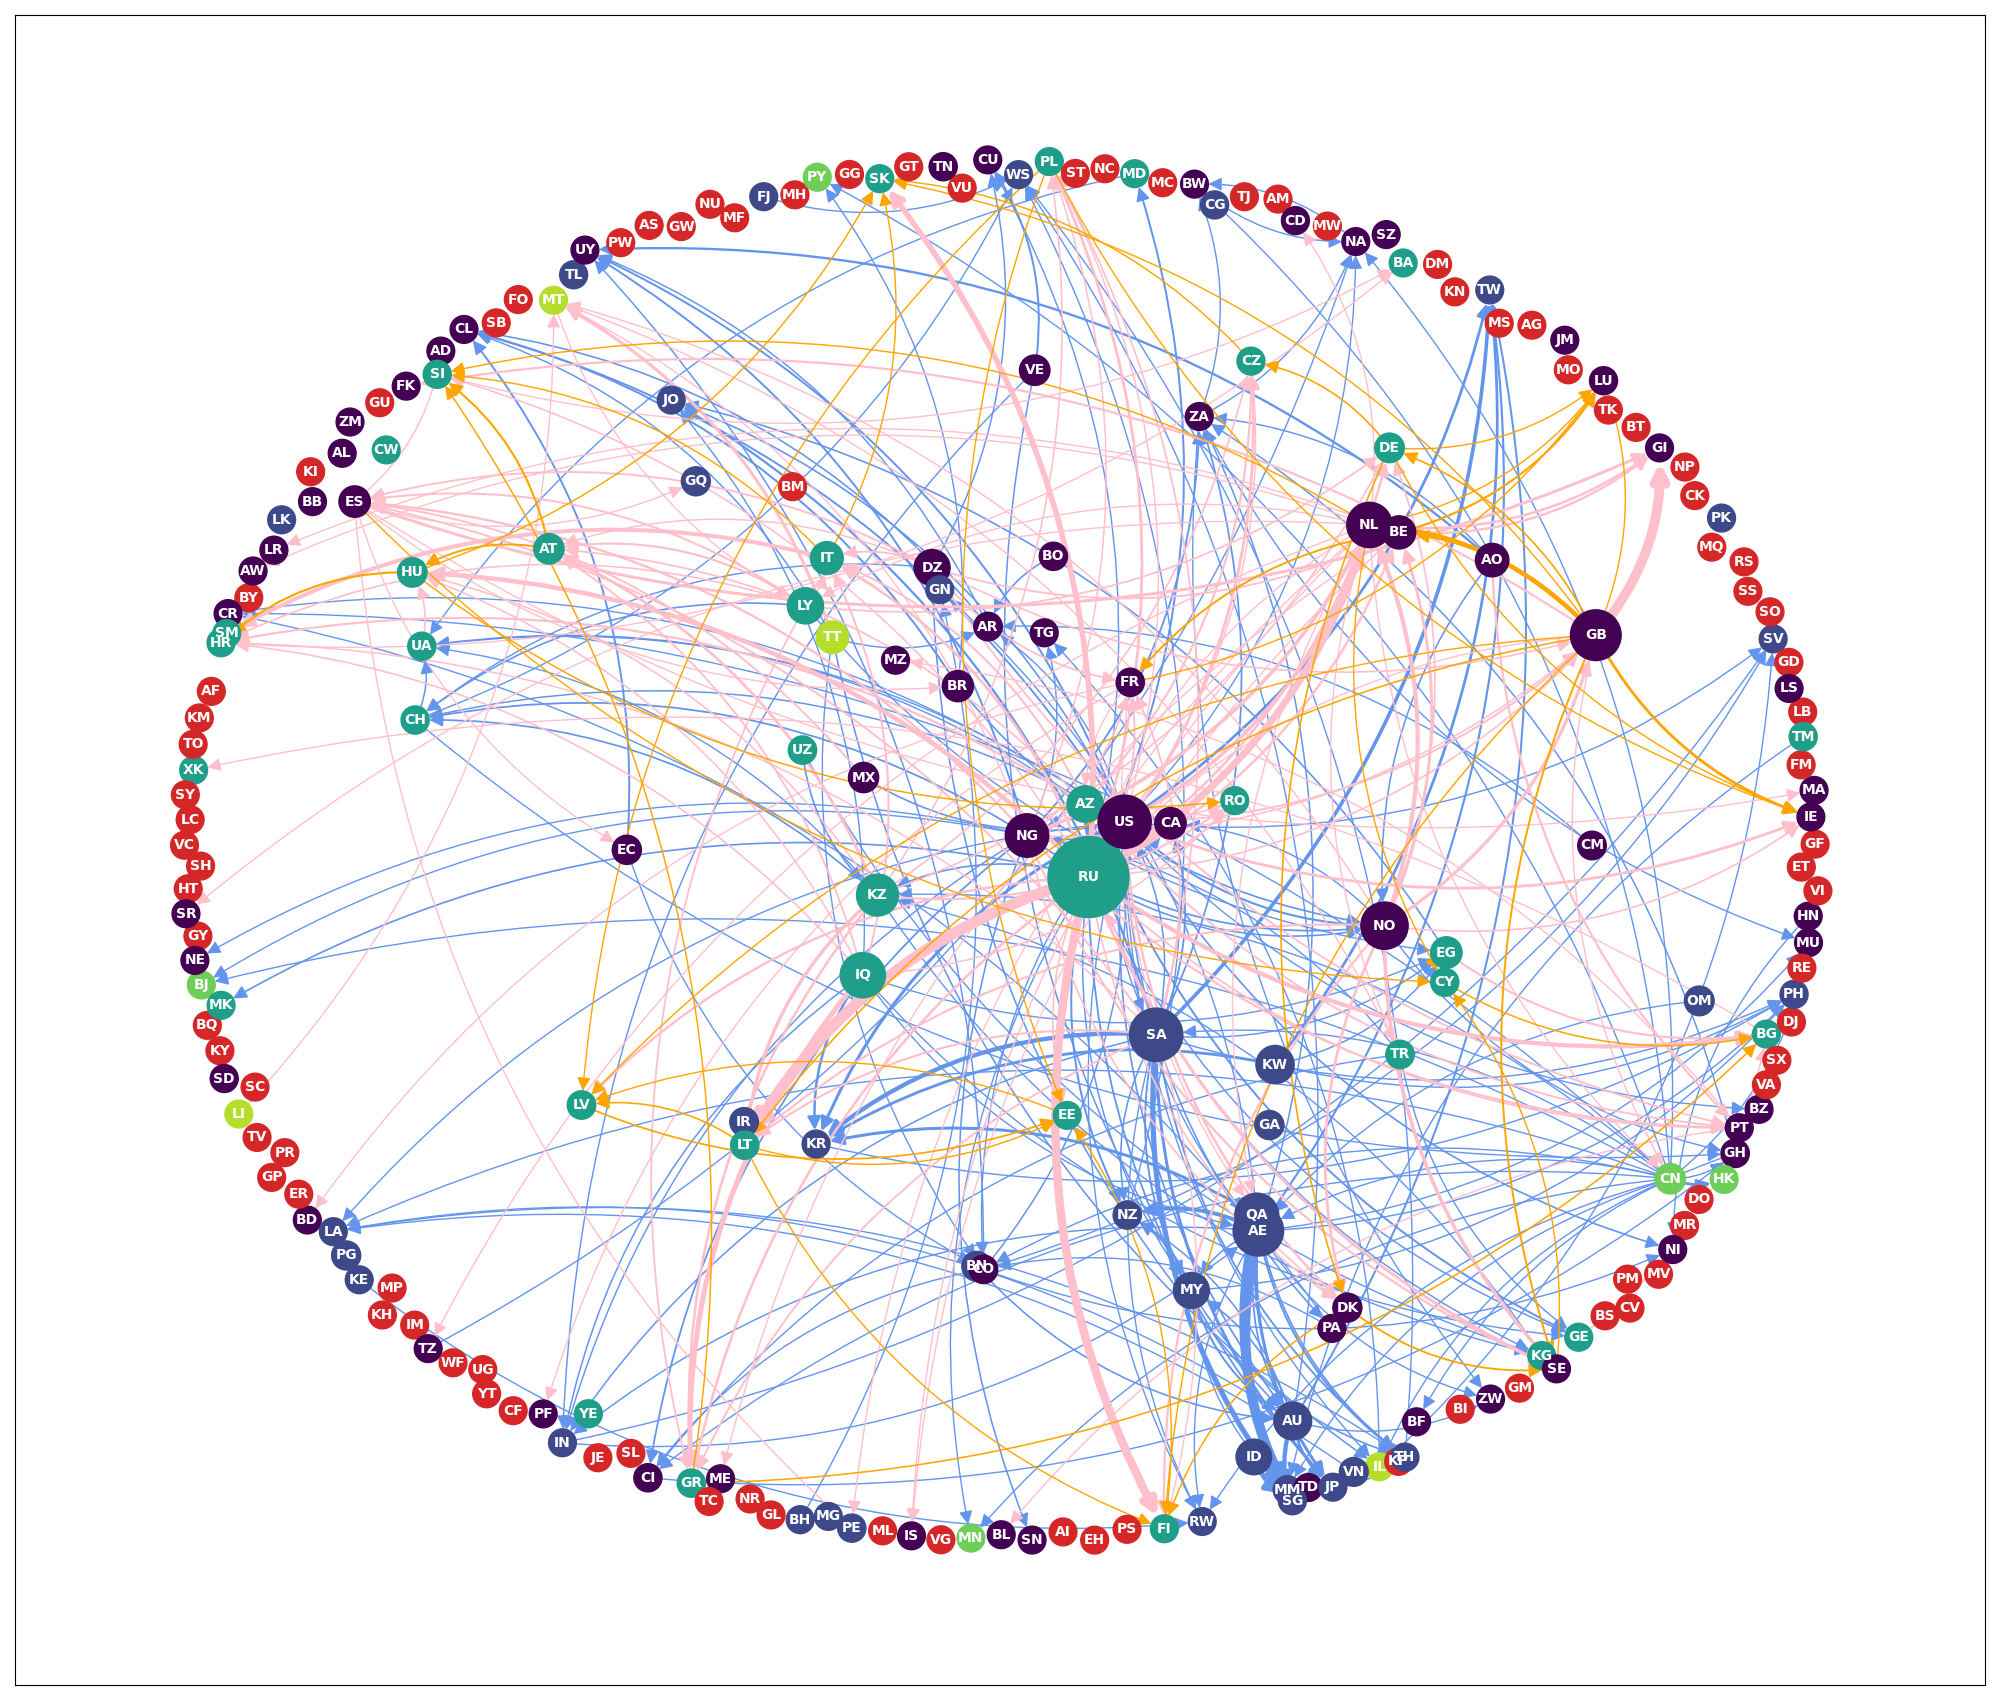
\includegraphics[width=\textwidth]{pics/full_y19_p06_force_147_lou.png}
        \caption{Louvain Method}
        \label{fig:gasnetworklou}
    \end{subfigure}
    \caption[Global trade network of \textit{Crude Petroleum and Natural Gas} in 2019, with communities.]{Global trade network of \textit{Crude Petroleum and Natural Gas} in 2019. The size of the node represents the \textit{out-strength} of that country. The color of the node corresponds to the block membership; the color of the edge is \textit{orange} for intra-EU exchanges, \textit{pink} for EU - non-EU exchanges and \textit{azure} for extra-EU exchanges. Only the top 10 import partnership for each country are shown.}
    \label{fig:gascommunities}
\end{figure}

